%%%%%%%%%%%%%%%%%%%%%%%%%%%%%%%%%%%%%%%%%
% Short Sectioned Assignment LaTeX Template Version 1.0 (5/5/12)
% This template has been downloaded from: http://www.LaTeXTemplates.com
% Original author:  Frits Wenneker (http://www.howtotex.com)
% License: CC BY-NC-SA 3.0 (http://creativecommons.org/licenses/by-nc-sa/3.0/)
%%%%%%%%%%%%%%%%%%%%%%%%%%%%%%%%%%%%%%%%%

% \documentclass[paper=a4, fontsize=11pt]{scrartcl} % A4 paper and 11pt font size
\documentclass[11pt, a4paper]{book}
\usepackage[T1]{fontenc} % Use 8-bit encoding that has 256 glyphs
\usepackage[utf8]{inputenc}
\usepackage{fourier} % Use the Adobe Utopia font for the document - comment this line to return to the LaTeX default
\usepackage{listings} % para insertar código con formato similar al editor
\usepackage[spanish, es-tabla]{babel} % Selecciona el español para palabras introducidas automáticamente, p.ej. "septiembre" en la fecha y especifica que se use la palabra Tabla en vez de Cuadro
\usepackage{url} % ,href} %para incluir URLs e hipervínculos dentro del texto (aunque hay que instalar href)
\usepackage{graphics,graphicx, float} %para incluir imágenes y colocarlas
\usepackage[gen]{eurosym} %para incluir el símbolo del euro
\usepackage{cite} %para incluir citas del archivo <nombre>.bib
\usepackage{enumerate}
\usepackage{hyperref}
\usepackage{graphicx}
\usepackage{tabularx}
\usepackage{booktabs}

\usepackage[table,xcdraw]{xcolor}
\hypersetup{
	colorlinks=true,	% false: boxed links; true: colored links
	linkcolor=black,	% color of internal links
	urlcolor=cyan		% color of external links
}
\renewcommand{\familydefault}{\sfdefault}
\usepackage{fancyhdr} % Custom headers and footers
\pagestyle{fancyplain} % Makes all pages in the document conform to the custom headers and footers
\fancyhead[L]{} % Empty left header
\fancyhead[C]{} % Empty center header
\fancyhead[R]{\minombre} % My name
\fancyfoot[L]{} % Empty left footer
\fancyfoot[C]{} % Empty center footer
\fancyfoot[R]{\thepage} % Page numbering for right footer
%\renewcommand{\headrulewidth}{0pt} % Remove header underlines
\renewcommand{\footrulewidth}{0pt} % Remove footer underlines
\setlength{\headheight}{13.6pt} % Customize the height of the header

\usepackage{titlesec, blindtext, color}
\definecolor{gray75}{gray}{0.75}
\newcommand{\hsp}{\hspace{20pt}}
\titleformat{\chapter}[hang]{\Huge\bfseries}{\thechapter\hsp\textcolor{gray75}{|}\hsp}{0pt}{\Huge\bfseries}
\setcounter{secnumdepth}{4}
\usepackage[Lenny]{fncychap}

\def\minombre{Raúl Soria González}
\def\tutor{Juan Manuel Fernández Luna}
\def\titulo{Social Gallery}
\def\subtitulo{Galería de arte para artistas independientes}
\def\subtituloingles{Art gallery for independent artists}

\graphicspath{{./img/}}


\begin{document}

	% Plantilla portada UGR
	\begin{titlepage}
\newlength{\centeroffset}
\setlength{\centeroffset}{-0.5\oddsidemargin}
\addtolength{\centeroffset}{0.5\evensidemargin}
\thispagestyle{empty}

\noindent\hspace*{\centeroffset}\begin{minipage}{\textwidth}

\centering

\includegraphics[width=0.9\textwidth]{logos/logo_ugr.jpg}\\[1.4cm]

\textsc{ \Large TRABAJO FIN DE GRADO\\[0.2cm]}
\textsc{ GRADO EN INGENIERIA INFORMATICA}\\[1cm]

{\Huge\bfseries Título \\}
\noindent\rule[-1ex]{\textwidth}{3pt}\\[3.5ex]
{\large\bfseries Subtítulo }
\end{minipage}

\vspace{2.5cm}
\noindent\hspace*{\centeroffset}
\begin{minipage}{\textwidth}
\centering

\textbf{Autor}\\ {Estudiante}\\[2.5ex]
\textbf{Director}\\ {Tutor(a)(es)}\\[2cm]

\includegraphics[width=0.3\textwidth]{logos/etsiit_logo.png}\\[0.1cm]
\textsc{Escuela Técnica Superior de Ingenierías Informática y de Telecomunicación}\\
\textsc{---}\\
Granada, Junio de 201x
\end{minipage}
\end{titlepage}


	% Plantilla prefacio UGR
	\thispagestyle{empty}

\begin{center}
{\large\bfseries \titulo \\ \subtitulo }\\
\end{center}
\begin{center}
\minombre\\
\end{center}

%\vspace{0.7cm}

\vspace{0.5cm}
\noindent\textbf{Palabras clave}: \textit{galería de arte, aplicación web, React, NodeJS, MySQL, Docker}
\vspace{0.7cm}

\noindent\textbf{Resumen}

\bigskip
El objetivo de este trabajo es el desarrollo de una aplicación web
que sirva como una galería de arte online en la que los artistas podrán publicar
sus obras para darlas a conocer. Los usuarios podrán ver y valorar las obras para poder
dar feedback a los artistas. El propósito de esta aplicación es que los artistas puedan
dar a conocer sus obras y que galerías de arte convencionales puedan descubrir nuevos
artistas para exponer sus obras.

\cleardoublepage

\begin{center}
	{\large\bfseries \titulo \\ \subtituloingles }\\
\end{center}
\begin{center}
	\minombre\\
\end{center}
\vspace{0.5cm}
\noindent\textbf{Keywords}: \textit{art gallery, web app, React, NodeJS, MySQL, Docker}
\vspace{0.7cm}

\noindent\textbf{Abstract}

\bigskip
The objective of this work is the development of a web application
that will serve as an online art gallery that serves as an online art
gallery where artists can publish their works to make them known.
Users will be able to view and rate the artworks in order to give
feedback to the artists. The purpose of this application is for artists
to be able to to make their works known and for conventional art
galleries to discover new artists to exhibit their works.


\cleardoublepage

\thispagestyle{empty}

\noindent\rule[-1ex]{\textwidth}{2pt}\\[4.5ex]

D. \textbf{\tutor}, catedrático del departamento de Ciencias de la
Computación e Inteligencia Artificial de la Universidad de Granada.

\vspace{0.5cm}

\textbf{Informo:}

\vspace{0.5cm}

Que el presente trabajo, titulado \textit{\textbf{\titulo}},
ha sido realizado bajo mi supervisión por \textbf{\minombre}, y autorizo la defensa de dicho trabajo ante el tribunal
que corresponda.

\vspace{0.5cm}

Y para que conste, expiden y firman el presente informe en Granada a Junio de 2023.

\vspace{1cm}

\textbf{El director: }

\vspace{5cm}

\noindent \textbf{\tutor}

\chapter*{Agradecimientos}






	% Índice de contenidos
	\newpage
	\tableofcontents

	% Índice de imágenes y tablas
	\newpage
	\listoffigures

	% Si hay suficientes se incluirá dicho índice
	\listoftables 
	\newpage

	% Introducción 
	% Estado del arte
	% 	1. Crítica al estado del arte
	% 	2. Propuesta
	\chapter{Introducción}

La tecnología está presente en casi todos los aspectos de nuestra vida a día de hoy. De hecho,
es un recurso que permite conectarnos con realidades que, de otra manera, quedarían
invisibilizadas. Sin embargo, en el mundo del arte nos encontramos con una circunstancia algo
diferente, ya que no se suele promocionar en los medios de comunicación a los que accede la
gran mayoría de la población. En este sentido, aunque entre sus amantes sí que existe un
mayor interés por seguir conociendo nuevos artistas, quizá para el resto de la población
general queda al margen. De esta manera, si una persona no tiene la iniciativa suficiente
como para conectarse día a día a las novedades, puede resultarle más complejo mantenerse
actualizado. 
 
\section{Motivación}  
 
En este contexto, surge la idea de desarrollar una aplicación web que permita a los artistas
publicar sus obras y promocionar su trabajo. Así, cualquier persona puede tener un fácil
acceso a las mismas, aumentando así la probabilidad de que más población se acerque a este
mundo. Además, para todos aquellos amantes del arte también es una forma de, en definitiva,
mejorar y reforzar la cercanía con los autores. Por ende, la principal motivación que inicia
este proyecto es crear una plataforma que permita promocionar las obras de pequeños artistas,
que sea intuitiva y fácil de usar para cualquier persona (ya sea quien enseña su trabajo o
quien disfruta conociéndolo). En definitiva, lo que se desea es acercar la cultura a la
población y viceversa, a través del uso de la tecnología.  
 
\section{Descripción del problema} 
 
Los artistas independientes suelen tener dificultades para darse a conocer y las herramientas
que tienen a su disposición para ello no son específicas para este fin. La mayoría de
artistas utilizan redes sociales como \textit{Instagram} \cite{instagram}, \textit{Facebook}
\cite{facebook} o \textit{Twitter} \cite{twitter} para publicar sus obras. Sin embargo, estas
aplicaciones no están diseñadas con este propósito; la mayoría de usuarios no las utilizan
para descubrir nuevos artistas sino para otros fines. Así, es difícil encontrar obras entre
la gran cantidad de contenido que se publica en estas redes.  
 
Por otro lado, las galerías de arte convencionales o estudios fotográficos no cuentan con
herramientas para poder descubrir nuevos artistas en sus exposiciones. En la mayoría de casos,
los artistas que muestran su trabajo en estos lugares ya tienen cierto reconocimiento y se
han dado a conocer anteriormente en otras galerías. Sin embargo, aquellos que se están
iniciando en este mundo y que quizá no han tenido las mismas oportunidades y/o facilidades
que sus colegas para acceder a estos recursos, a veces simplemente por mera cuestión de
suerte, tienen más dificultades para empezar a trabajar de lo que tanto les gusta.  

Además, los grandes centros urbanos suelen ser los lugares que alojan eventos culturales para
promocionar el arte independiente. Sin embargo, a día de hoy es más difícil encontrar esta
misma situación en ciudades y pueblos más pequeños. En ellos, el único medio que tienen las
personas para conocer nuevos artistas es a través de internet, pero, como se ha descrito
anteriormente, no existe ninguna plataforma específica para este fin.

\section{Objetivos}

El propósito de este proyecto es el desarrollo de una aplicación web realizando todo
el proceso de ingeniería del software. Se realizará la fase de planificación, análisis,
diseño e implementación de la aplicación.

También se prentende aprender a utilizar tecnologías para el desarrollo de aplicaciones
web, enfocando el proyecto a un desarrollo full-stack. Se utilizarán tecnologías de las
que no se tenga mucho conocimiento y se quiera aprender como \textit{React} \cite{react}
o \textit{NodeJS} \cite{nodejs}.

Además de aprender a utilizar estas tecnologías, se pretende aprender a utilizar
de una forma más avanzada \textit{Docker} \cite{docker} y \textit{docker-compose}
\cite{docker-compose} para conectar las distintas partes de la aplicación.

Por último, se pretende desarrollar la aplicación de manera que sea intuitiva y fácil
de usar por personas que no posean grandes conocimientos informáticos. La mayoría de
las aplicaciones web que existen están enfocadas a un público con conocimientos o son
poco intuitivas para el usuario final. Para ello será importante realizar un buen
diseño de la interfaz de usuario que sea atractivo y fácil de usar.

\section{Revisión del estado del Arte}

{ \setlength{\parskip}{7mm} % Customize the space between paragraphs
Existen varias aplicaciones web que sirven como galerías de arte online, pero la mayoría
de ellas están enfocadas a la venta de obras de arte y no tanto a la exposición de obras
y promoción de las mismas.

Un ejemplo de esto es la aplicación web \textit{Artfinder} \cite{artfinder}, que permite
a los artistas vender sus obras a través de la plataforma. Sin embargo, no permite a los
usuarios valorar las obras ni dar feedback a los artistas, tampoco poder encontrar las obras
con mayor puntuación.

Otra aplicación es \textit{Singulart} \cite{singulart}, que también permite a los artistas
subir sus obras, aunque para ello, primero deben postular y luego ser aceptados por el equipo
de la plataforma. Además, la página advierte a los artistas que el proceso de aceptación
es muy largo ya que reciben demasiadas solicitudes. Por otro lado, los usuarios tampoco
pueden valorar las obras ni dejar sus comentarios. La página actúa como un \textit{e-commerce}
o tienda online, en la que los artistas ponen a la venta sus obras y los usuarios pueden
buscar obras y comprarlas.

En cuanto a las aplicaciones web que permiten a los usuarios valorar las obras, se encuentra
\textit{ArtStation} \cite{artstation}, que es una plataforma para que los artistas suban
sus obras y los usuarios puedan valorarlas. Sin embargo, esta plataforma está enfocada
a artistas digitales solamente. Además, la interfaz está muy sobrecargada y no es intuitiva
para los usuarios.

En definitiva, no hay una gran oferta de aplicaciones web que permitan a los artistas
independientes publicar sus obras para darse a conocer y a los usuarios valorarlas. La
mayoría de aplicaciones web que existen están enfocadas a la venta de obras de arte y no
tanto a la exposición de obras y promoción de los artistas.
}

	% Descripción del problema y hasta donde se llega
	\chapter{Planificación}

\section{Metodología utilizada}


\section{Temporización}

\section{Presupuesto}


	% Análisis del problema
	% 1. Análisis de requisitos
	% 2. Análisis de las soluciones
	% 3. Solucion propuesta
	% 4. Análisis de seguridad
	\chapter{Análisis del problema}
En este capítulo vamos a realizar un análisis de las funcionalidades que debe cumplir
nuestra aplicación. Para ello, vamos a definir los requisitos funcionales,
no funcionales y de información que debe cumplir. Además, vamos a definir los
casos de uso que se van a dar en nuestra aplicación con sus respectivos diagramas.

\section{Requisitos}
Los actores que van a interactuar con nuestra aplicación son los siguientes:

\begin{itemize}
    \item \textbf{Usuario:} Usuario no registrado en la aplicación. Tendrá funcionalidades
    básicas.
    \item \textbf{Usuario registrado:} Usuario registrado en la aplicación. Tendrá
    acceso a más funcionalidades que el usuario no registrado.
    \item \textbf{Artista:} Usuario registrado con rol de artista. Podrá subir sus
    obras a la aplicación.
    \item \textbf{Administrador:} Usuario registrado con rol de administrador. Podrá
    realizar tareas de administración.
\end{itemize}

\subsection{Requisitos funcionales}
A continuación se van a definir los requisitos funcionales que debe cumplir nuestra
aplicación.

\begin{itemize}
    \item \textbf{RF-1:} Registrarse en la aplicación
    \begin{itemize}
        \item \textbf{RF-1.1:} Registrarse como usuario
        \item \textbf{RF-1.2:} Registrarse como artista
    \end{itemize}
    \item \textbf{RF-2:} Iniciar sesión
    \item \textbf{RF-3:} Eliminar usuario
    \begin{itemize}
        \item \textbf{RF-3.1:} Borrar cuenta como usuario registrado
        \item \textbf{RF-3.2:} Borrar cuenta como administrador
    \end{itemize}
    \item \textbf{RF-4:} Mostrar galería
    \item \textbf{RF-5:} Subir obra en galería
    \item \textbf{RF-6:} Mostrar detalles de obra
    \item \textbf{RF-7:} Valorar obra
    \item \textbf{RF-8:} Mostrar valoraciones de obra
    \item \textbf{RF-9:} Ordenar obras por fecha
    \begin{itemize}
        \item \textbf{RF-9.1:} Ordenar obras fecha descendente
        \item \textbf{RF-9.2:} Ordenar obras fecha ascendente
    \end{itemize}
    \item \textbf{RF-10:} Ordenar obras por valoración
    \begin{itemize}
        \item \textbf{RF-10.1:} Ordenar obras valoración descendente
        \item \textbf{RF-10.2:} Ordenar obras valoración ascendente
    \end{itemize}
    \item \textbf{RF-11:} Filtrar obras por autor
    \item \textbf{RF-12:} Eliminar obra
    \begin{itemize}
        \item \textbf{RF-12.1:} Eliminar obra como artista
        \item \textbf{RF-12.2:} Eliminar obra como administrador
    \end{itemize}
    \item \textbf{RF-13:} Eliminar valoración
    \begin{itemize}
        \item \textbf{RF-13.1:} Eliminar valoración como usuario registrado
        \item \textbf{RF-13.2:} Eliminar valoración como administrador
    \end{itemize}
    \item \textbf{RF-14:} Cerrar sesión
\end{itemize}

\subsection{Requisitos no funcionales}
En cuanto a los requisitos no funcionales, se van a definir los siguientes:

\begin{itemize}
    \item \textbf{RNF-1:} Eficiencia
    \begin{itemize}
        \item \textbf{RNF-1.1:} Toda funcionalidad ha de responder al usuario en menos
        de 5 segundos.
        \item \textbf{RNF-1.2:} La aplicación ha de operar correctamente con hasta 100
        sesiones concurrentes.
        \item \textbf{RNF-1.3:} Los datos modificados en la base de datos tienen que
        estar actualizados en menos de 5 segundos.
    \end{itemize}
    \item \textbf{RNF-2:} Seguridad lógica y de datos
    \begin{itemize}
        \item \textbf{RNF-2.1:} Los permisos de usuario administarador solo pueden ser
        modificados por otro usuario administrador.
        \item \textbf{RNF-2.2:} La aplicación se desarrollará aplicando patrones de
        programación que aumenten la seguirdad de los datos.
        \item \textbf{RNF-2.3:} Los datos sensibles de los usuarios serán encriptados
        antes de almacenarse en la base de datos.
    \end{itemize}
    \item \textbf{RNF-3:} Usabilidad
    \begin{itemize}
        \item \textbf{RNF-3.1:} La aplicación ha de ser intuitiva y fácil de usar por
        personas que no posean grandes conocimientos informáticos.
        \item \textbf{RNF-3.2:} La aplicación cumplirá con los estándares mínimos de
        accesibilidad.
        \item \textbf{RNF-3.3:} Los mensajes de error que proporcione la aplicación
        han de ser informativos y orientados al usuario final.
        \item \textbf{RNF-3.4:} La aplicación ha de ser compatible con los navegadores
        más utilizados.
        \item \textbf{RNF-3.5:} La aplicación ha de tener un diseño responsive, adaptándose
        a diversos tamaños de pantalla y dispositivos.
        \item \textbf{RNF-3.6:} Las imágenes se almacenarán en formato \textit{JPEG} o
        \textit{PNG}.
    \end{itemize}
\end{itemize}

\subsection{Requisitos de información}
Ahora se van a definir los requisitos de información que debe cumplir nuestra
aplicación.

\begin{itemize}
    \item \textbf{RI-1:} Usuario
    \begin{itemize}
        \item \textbf{RI-1.1:} Nombre
        \item \textbf{RI-1.2:} Apellidos
        \item \textbf{RI-1.3:} Correo electrónico
        \item \textbf{RI-1.4:} Contraseña
        \item \textbf{RI-1.5:} Es o no artista
        \item \textbf{RI-1.6:} Es o no administrador
    \end{itemize}
    \item \textbf{RI-2:} Obra
    \begin{itemize}
        \item \textbf{RI-2.1:} Título
        \item \textbf{RI-2.2:} Descripción
        \item \textbf{RI-2.3:} Tipo de obra
        \item \textbf{RI-2.4:} Fecha de creación
        \item \textbf{RI-2.5:} Valoración media
        \item \textbf{RI-2.6:} Autor
        \item \textbf{RI-2.7:} Archivo
    \end{itemize}
    \item \textbf{RI-3:} Valoración
    \begin{itemize}
        \item \textbf{RI-3.1:} Valoración
        \item \textbf{RI-3.2:} Comentario
    \end{itemize}
\end{itemize}

\subsection{Descripción de los requisitos}
A continuación se van a realizar las tablas de descripción de los requisitos funcionales.

\begin{table}[H]
    \centering
    \begin{tabular}{|p{3cm}|p{8cm}|}
        \hline
        \rowcolor{lightgray}
        \textbf{Detalle} & \textbf{Descripción} \\
        \hline
        \textbf{RF\#} & 1.1 \\
        \hline
        \textbf{Nombre} & Registrarse como usuario registrado \\
        \hline
        \textbf{Descripción} & Un usuario podrá registrarse en la aplicación \\
        \hline
        \textbf{Entrada} &
        Agente externo: Usuario
        
        Requisito de datos de entrada: RDE-1.1 \\
        \hline
        \textbf{BD} &
        Requisito de datos de lectura: ninguno
        
        Requisito de datos de escritura: RDW-1.1 \\
        \hline
        \textbf{Salida} & Requisito de datos de salida: ninguno \\
        \hline
        \textbf{RDE-1.1} & Datos de entrada para el registro de un usuario:
            \begin{itemize}
                \item Datos de usuario RI-1
            \end{itemize} \\
        \hline
        \textbf{RDW-1.1} & Datos almacenados de un usuario:
            \begin{itemize}
                \item Datos de usuario RI-1
            \end{itemize} \\
        \hline
    \end{tabular}
    \caption{Descripción del requisito funcional RF-1.1}
    \label{tab:rf-1-1}
\end{table}

\begin{table}[H]
    \centering
    \begin{tabular}{|p{3cm}|p{8cm}|}
        \hline
        \rowcolor{lightgray}
        \textbf{Detalle} & \textbf{Descripción} \\
        \hline
        \textbf{RF\#} & 1.2 \\
        \hline
        \textbf{Nombre} & Registrarse como artista \\
        \hline
        \textbf{Descripción} & Un usuario podrá registrarse en la aplicación como artista \\
        \hline
        \textbf{Entrada} &
        Agente externo: Usuario
        
        Requisito de datos de entrada: RDE-1.2 \\
        \hline
        \textbf{BD} &
        Requisito de datos de lectura: ninguno
        
        Requisito de datos de escritura: RDW-1.2 \\
        \hline
        \textbf{Salida} & Requisito de datos de salida: ninguno \\
        \hline
        \textbf{RDE-1.2} & Datos de entrada para el registro de un usuario como artista:
            \begin{itemize}
                \item Usuario RI-1
            \end{itemize} \\
        \hline
        \textbf{RDW-1.2} & Datos almacenados de un usuario:
            \begin{itemize}
                \item Usuario RI-1
            \end{itemize} \\
        \hline
    \end{tabular}
    \caption{Descripción del requisito funcional RF-1.2}
    \label{tab:rf-1-2}
\end{table}

\begin{table}[H]
    \centering
    \begin{tabular}{|p{3cm}|p{8cm}|}
        \hline
        \rowcolor{lightgray}
        \textbf{Detalle} & \textbf{Descripción} \\
        \hline
        \textbf{RF\#} & 2 \\
        \hline
        \textbf{Nombre} & Iniciar sesión \\
        \hline
        \textbf{Descripción} & Un usuario podrá iniciar sesión en la aplicación \\
        \hline
        \textbf{Entrada} &
        Agente externo: Usuario
        
        Requisito de datos de entrada: RDE-2 \\
        \hline
        \textbf{BD} &
        Requisito de datos de lectura: RDR-2
        
        Requisito de datos de escritura: ninguno \\
        \hline
        \textbf{Salida} & Requisito de datos de salida: ninguno \\
        \hline
        \textbf{RDE-2} & Datos de entrada para iniciar sesión:
            \begin{itemize}
                \item Correo electrónico RI-1.3
                \item Contraseña RI-1.4
            \end{itemize} \\
        \hline
        \textbf{RDR-2} & Datos de lectura de un usuario:
            \begin{itemize}
                \item Usuario RI-1
            \end{itemize} \\
        \hline
    \end{tabular}
    \caption{Descripción del requisito funcional RF-2}
    \label{tab:rf-2}
\end{table}

\begin{table}[H]
    \centering
    \begin{tabular}{|p{3cm}|p{8cm}|}
        \hline
        \rowcolor{lightgray}
        \textbf{Detalle} & \textbf{Descripción} \\
        \hline
        \textbf{RF\#} & 3.1 \\
        \hline
        \textbf{Nombre} & Borrar cuenta como usuario registrado \\
        \hline
        \textbf{Descripción} & Un usuario registrado podrá borrar su cuenta \\
        \hline
        \textbf{Entrada} &
        Agente externo: Usuario registrado
        
        Requisito de datos de entrada: ninguno \\
        \hline
        \textbf{BD} &
        Requisito de datos de lectura: RDR-3.1
        
        Requisito de datos de escritura: RDW-3.1 \\
        \hline
        \textbf{Salida} & Requisito de datos de salida: ninguno \\
        \hline
        \textbf{RDR-3.1} & Datos de lectura para borrar un usuario:
            \begin{itemize}
                \item Usuario RI-1
                \item Obras del usuario RI-2
            \end{itemize} \\
        \hline
        \textbf{RDW-3.1} & Datos de escritura de un usuario:
            \begin{itemize}
                \item Eliminar usuario RI-1
                \item Eliminar obras del usuario RI-2
            \end{itemize} \\
        \hline
    \end{tabular}
    \caption{Descripción del requisito funcional RF-3.1}
    \label{tab:rf-3-1}
\end{table}

\begin{table}[H]
    \centering
    \begin{tabular}{|p{3cm}|p{8cm}|}
        \hline
        \rowcolor{lightgray}
        \textbf{Detalle} & \textbf{Descripción} \\
        \hline
        \textbf{RF\#} & 3.2 \\
        \hline
        \textbf{Nombre} & Borrar cuenta como administrador \\
        \hline
        \textbf{Descripción} & Un administrador podrá borrar la cuenta de un usuario \\
        \hline
        \textbf{Entrada} &
        Agente externo: Administrador
        
        Requisito de datos de entrada: RDE-3.2 \\
        \hline
        \textbf{BD} &
        Requisito de datos de lectura: RDR-3.2
        
        Requisito de datos de escritura: RDW-3.2 \\
        \hline
        \textbf{Salida} & Requisito de datos de salida: ninguno \\
        \hline
        \textbf{RDE-3.2} & Datos de entrada para borrar un usuario:
            \begin{itemize}
                \item Usuario RI-1
            \end{itemize} \\
        \hline
        \textbf{RDR-3.2} & Datos de lectura para borrar un usuario:
            \begin{itemize}
                \item Usuario RI-1
                \item Obras del usuario RI-2
            \end{itemize} \\
        \hline
        \textbf{RDW-3.2} & Datos de escritura para borrar un usuario:
            \begin{itemize}
                \item Eliminar usuario RI-1
                \item Eliminar obras del usuario RI-2
            \end{itemize} \\
        \hline
    \end{tabular}
    \caption{Descripción del requisito funcional RF-3.2}
    \label{tab:rf-3-2}
\end{table}

\begin{table}[H]
    \centering
    \begin{tabular}{|p{3cm}|p{8cm}|}
        \hline
        \rowcolor{lightgray}
        \textbf{Detalle} & \textbf{Descripción} \\
        \hline
        \textbf{RF\#} & 4 \\
        \hline
        \textbf{Nombre} & Mostrar galería \\
        \hline
        \textbf{Descripción} & Mostrar todas las obras de la galería \\
        \hline
        \textbf{Entrada} &
        Agente externo: Usuario
        
        Requisito de datos de entrada: RDE-4 \\
        \hline
        \textbf{BD} &
        Requisito de datos de lectura: RDR-4
        
        Requisito de datos de escritura: ninguno \\
        \hline
        \textbf{Salida} & Requisito de datos de salida: RDS-4 \\
        \hline
        \textbf{RDE-4} & Datos de entrada para mostrar la galería:
            \begin{itemize}
                \item Tipo de obra RI-2.3
            \end{itemize} \\
        \hline
        \textbf{RDR-4} & Datos de lectura para mostrar la galería:
            \begin{itemize}
                \item Obras RI-2
            \end{itemize} \\
        \hline
        \textbf{RDS-4} & Datos de salida para mostrar la galería:
            \begin{itemize}
                \item Obras RI-2
            \end{itemize} \\
        \hline
    \end{tabular}
    \caption{Descripción del requisito funcional RF-4}
    \label{tab:rf-4}
\end{table}

\begin{table}[H]
    \centering
    \begin{tabular}{|p{3cm}|p{8cm}|}
        \hline
        \rowcolor{lightgray}
        \textbf{Detalle} & \textbf{Descripción} \\
        \hline
        \textbf{RF\#} & 5 \\
        \hline
        \textbf{Nombre} & Subir obra en galería \\
        \hline
        \textbf{Descripción} & Un artista podrá subir una obra a la galería \\
        \hline
        \textbf{Entrada} &
        Agente externo: Artista
        
        Requisito de datos de entrada: RDE-5 \\
        \hline
        \textbf{BD} &
        Requisito de datos de lectura: ninguno
        
        Requisito de datos de escritura: RDW-5 \\
        \hline
        \textbf{Salida} & Requisito de datos de salida: ninguno \\
        \hline
        \textbf{RDE-5} & Datos de entrada para subir una obra:
            \begin{itemize}
                \item Obra RI-2
            \end{itemize} \\
        \hline
        \textbf{RDW-5} & Datos de escritura para subir una obra:
            \begin{itemize}
                \item Obra RI-2
            \end{itemize} \\
        \hline
    \end{tabular}
    \caption{Descripción del requisito funcional RF-5}
    \label{tab:rf-5}
\end{table}

\begin{table}[H]
    \centering
    \begin{tabular}{|p{3cm}|p{8cm}|}
        \hline
        \rowcolor{lightgray}
        \textbf{Detalle} & \textbf{Descripción} \\
        \hline
        \textbf{RF\#} & 6 \\
        \hline
        \textbf{Nombre} & Mostrar detalles de obra \\
        \hline
        \textbf{Descripción} & Mostrar los detalles de una obra \\
        \hline
        \textbf{Entrada} &
        Agente externo: Usuario
        
        Requisito de datos de entrada: RDE-6 \\
        \hline
        \textbf{BD} &
        Requisito de datos de lectura: RDR-6
        
        Requisito de datos de escritura: ninguno \\
        \hline
        \textbf{Salida} & Requisito de datos de salida: RDS-6 \\
        \hline
        \textbf{RDE-6} & Datos de entrada para mostrar los detalles de una obra:
            \begin{itemize}
                \item Obra RI-2
            \end{itemize} \\
        \hline
        \textbf{RDR-6} & Datos de lectura para mostrar los detalles de una obra:
            \begin{itemize}
                \item Contenido obra RI-2.7
            \end{itemize} \\
        \hline
        \textbf{RDS-6} & Datos de salida para mostrar los detalles de una obra:
            \begin{itemize}
                \item Contenido obra RI-2.7
            \end{itemize} \\
        \hline
    \end{tabular}
    \caption{Descripción del requisito funcional RF-6}
    \label{tab:rf-6}
\end{table}

\begin{table}[H]
    \centering
    \begin{tabular}{|p{3cm}|p{8cm}|}
        \hline
        \rowcolor{lightgray}
        \textbf{Detalle} & \textbf{Descripción} \\
        \hline
        \textbf{RF\#} & 7 \\
        \hline
        \textbf{Nombre} & Valorar obra \\
        \hline
        \textbf{Descripción} & Un usuario registrado podrá valorar una obra con
        una puntuación y un comentario opcionalmente \\
        \hline
        \textbf{Entrada} &
        Agente externo: Usuario registrado
        
        Requisito de datos de entrada: RDE-7 \\
        \hline
        \textbf{BD} &
        Requisito de datos de lectura: ninguno
        
        Requisito de datos de escritura: RDW-7 \\
        \hline
        \textbf{Salida} & Requisito de datos de salida: ninguno \\
        \hline
        \textbf{RDE-7} & Datos de entrada para valorar una obra:
            \begin{itemize}
                \item Obra RI-2
                \item Valoración RI-3.1
                \item Comentario RI-3.2
            \end{itemize} \\
        \hline
        \textbf{RDW-7} & Datos de escritura para valorar una obra:
            \begin{itemize}
                \item Valoración RI-3
            \end{itemize} \\
        \hline
    \end{tabular}
    \caption{Descripción del requisito funcional RF-7}
    \label{tab:rf-7}
\end{table}

\begin{table}[H]
    \centering
    \begin{tabular}{|p{3cm}|p{8cm}|}
        \hline
        \rowcolor{lightgray}
        \textbf{Detalle} & \textbf{Descripción} \\
        \hline
        \textbf{RF\#} & 8 \\
        \hline
        \textbf{Nombre} & Mostrar valoraciones de obra \\
        \hline
        \textbf{Descripción} & Mostrar las valoraciones de una obra \\
        \hline
        \textbf{Entrada} &
        Agente externo: Usuario
        
        Requisito de datos de entrada: RDE-8 \\
        \hline
        \textbf{BD} &
        Requisito de datos de lectura: RDR-8
        
        Requisito de datos de escritura: ninguno \\
        \hline
        \textbf{Salida} & Requisito de datos de salida: RDS-8 \\
        \hline
        \textbf{RDE-8} & Datos de entrada para mostrar las valoraciones de una obra:
            \begin{itemize}
                \item Obra RI-2
            \end{itemize} \\
        \hline
        \textbf{RDR-8} & Datos de lectura para mostrar las valoraciones de una obra:
            \begin{itemize}
                \item Valoraciones RI-3
            \end{itemize} \\
        \hline
        \textbf{RDS-8} & Datos de salida para mostrar las valoraciones de una obra:
            \begin{itemize}
                \item Valoraciones RI-3
            \end{itemize} \\
        \hline
    \end{tabular}
    \caption{Descripción del requisito funcional RF-8}
    \label{tab:rf-8}
\end{table}

\begin{table}[H]
    \centering
    \begin{tabular}{|p{3cm}|p{8cm}|}
        \hline
        \rowcolor{lightgray}
        \textbf{Detalle} & \textbf{Descripción} \\
        \hline
        \textbf{RF\#} & 9.1 \\
        \hline
        \textbf{Nombre} & Ordenar obras por fecha descendente \\
        \hline
        \textbf{Descripción} & Un usuario podrá visualizar las obras ordenadas
        por fecha de creación de forma descendente \\
        \hline
        \textbf{Entrada} &
        Agente externo: Usuario
        
        Requisito de datos de entrada: ninguno \\
        \hline
        \textbf{BD} &
        Requisito de datos de lectura: RDR-9.1
        
        Requisito de datos de escritura: ninguno \\
        \hline
        \textbf{Salida} & Requisito de datos de salida: RDS-9.1 \\
        \hline
        \textbf{RDR-9.1} & Datos de lectura para mostrar las obras ordenadas por fecha
        de creación de forma descendente:
            \begin{itemize}
                \item Obras RI-2
                \item Fecha de creación RI-2.4
            \end{itemize} \\
        \hline
        \textbf{RDS-9.1} & Datos de salida para mostrar las obras ordenadas por fecha
        de creación de forma descendente:
            \begin{itemize}
                \item Obras RI-2
            \end{itemize} \\
        \hline
    \end{tabular}
    \caption{Descripción del requisito funcional RF-9.1}
    \label{tab:rf-9-1}
\end{table}

\begin{table}[H]
    \centering
    \begin{tabular}{|p{3cm}|p{8cm}|}
        \hline
        \rowcolor{lightgray}
        \textbf{Detalle} & \textbf{Descripción} \\
        \hline
        \textbf{RF\#} & 9.2 \\
        \hline
        \textbf{Nombre} & Ordenar obras por fecha ascendente \\
        \hline
        \textbf{Descripción} & Un usuario podrá visualizar las obras ordenadas
        por fecha de creación de forma ascendente \\
        \hline
        \textbf{Entrada} &
        Agente externo: Usuario
        
        Requisito de datos de entrada: ninguno \\
        \hline
        \textbf{BD} &
        Requisito de datos de lectura: RDR-9.2
        
        Requisito de datos de escritura: ninguno \\
        \hline
        \textbf{Salida} & Requisito de datos de salida: RDS-9.2 \\
        \hline
        \textbf{RDR-9.2} & Datos de lectura para mostrar las obras ordenadas por fecha
        de creación de forma ascendente:
            \begin{itemize}
                \item Obras RI-2
                \item Fecha de creación RI-2.4
            \end{itemize} \\
        \hline
        \textbf{RDS-9.2} & Datos de salida para mostrar las obras ordenadas por fecha
        de creación de forma ascendente:
            \begin{itemize}
                \item Obras RI-2
            \end{itemize} \\
        \hline
    \end{tabular}
    \caption{Descripción del requisito funcional RF-9.2}
    \label{tab:rf-9-2}
\end{table}

\begin{table}[H]
    \centering
    \begin{tabular}{|p{3cm}|p{8cm}|}
        \hline
        \rowcolor{lightgray}
        \textbf{Detalle} & \textbf{Descripción} \\
        \hline
        \textbf{RF\#} & 10.1 \\
        \hline
        \textbf{Nombre} & Ordenar obras por valoración descendente \\
        \hline
        \textbf{Descripción} & Un usuario podrá visualizar las obras ordenadas
        por valoración de forma descendente \\
        \hline
        \textbf{Entrada} &
        Agente externo: Usuario
        
        Requisito de datos de entrada: ninguno \\
        \hline
        \textbf{BD} &
        Requisito de datos de lectura: RDR-10.1
        
        Requisito de datos de escritura: ninguno \\
        \hline
        \textbf{Salida} & Requisito de datos de salida: RDS-10.1 \\
        \hline
        \textbf{RDR-10.1} & Datos de lectura para mostrar las obras ordenadas por valoración
        de forma descendente:
            \begin{itemize}
                \item Obras RI-2
                \item Valoración media RI-2.5
            \end{itemize} \\
        \hline
        \textbf{RDS-10.1} & Datos de salida para mostrar las obras ordenadas por valoración
        de forma descendente:
            \begin{itemize}
                \item Obras RI-2
            \end{itemize} \\
        \hline
    \end{tabular}
    \caption{Descripción del requisito funcional RF-10.1}
    \label{tab:rf-10-1}
\end{table}

\begin{table}[H]
    \centering
    \begin{tabular}{|p{3cm}|p{8cm}|}
        \hline
        \rowcolor{lightgray}
        \textbf{Detalle} & \textbf{Descripción} \\
        \hline
        \textbf{RF\#} & 10.2 \\
        \hline
        \textbf{Nombre} & Ordenar obras por valoración ascendente \\
        \hline
        \textbf{Descripción} & Un usuario podrá visualizar las obras ordenadas
        por valoración de forma ascendente \\
        \hline
        \textbf{Entrada} &
        Agente externo: Usuario
        
        Requisito de datos de entrada: ninguno \\
        \hline
        \textbf{BD} &
        Requisito de datos de lectura: RDR-10.2
        
        Requisito de datos de escritura: ninguno \\
        \hline
        \textbf{Salida} & Requisito de datos de salida: RDS-10.2 \\
        \hline
        \textbf{RDR-10.2} & Datos de lectura para mostrar las obras ordenadas por valoración
        de forma ascendente:
            \begin{itemize}
                \item Obras RI-2
                \item Valoración media RI-2.5
            \end{itemize} \\
        \hline
        \textbf{RDS-10.2} & Datos de salida para mostrar las obras ordenadas por valoración
        de forma ascendente:
            \begin{itemize}
                \item Obras RI-2
            \end{itemize} \\
        \hline
    \end{tabular}
    \caption{Descripción del requisito funcional RF-10.2}
    \label{tab:rf-10-2}
\end{table}

\begin{table}[H]
    \centering
    \begin{tabular}{|p{3cm}|p{8cm}|}
        \hline
        \rowcolor{lightgray}
        \textbf{Detalle} & \textbf{Descripción} \\
        \hline
        \textbf{RF\#} & 11 \\
        \hline
        \textbf{Nombre} & Filtrar obras por autor \\
        \hline
        \textbf{Descripción} & Un usuario podrá visualizar las obras de un autor
        concreto \\
        \hline
        \textbf{Entrada} &
        Agente externo: Usuario
        
        Requisito de datos de entrada: RDE-11 \\
        \hline
        \textbf{BD} &
        Requisito de datos de lectura: RDR-11
        
        Requisito de datos de escritura: ninguno \\
        \hline
        \textbf{Salida} & Requisito de datos de salida: RDS-11 \\
        \hline
        \textbf{RDE-11} & Datos de entrada para mostrar las obras de un autor:
            \begin{itemize}
                \item Autor RI-2.6
            \end{itemize} \\
        \hline
        \textbf{RDR-11} & Datos de lectura para mostrar las obras de un autor:
            \begin{itemize}
                \item Obras RI-2
                \item Autor RI-2.6
            \end{itemize} \\
        \hline
        \textbf{RDS-11} & Datos de salida para mostrar las obras de un autor:
            \begin{itemize}
                \item Obras RI-2
            \end{itemize} \\
        \hline
    \end{tabular}
    \caption{Descripción del requisito funcional RF-11}
    \label{tab:rf-11}
\end{table}

\begin{table}[H]
    \centering
    \begin{tabular}{|p{3cm}|p{8cm}|}
        \hline
        \rowcolor{lightgray}
        \textbf{Detalle} & \textbf{Descripción} \\
        \hline
        \textbf{RF\#} & 12.1 \\
        \hline
        \textbf{Nombre} & Eliminar obra como artista \\
        \hline
        \textbf{Descripción} & Un artista podrá eliminar una obra suya \\
        \hline
        \textbf{Entrada} &
        Agente externo: Artista

        Requisito de datos de entrada: RDE-12.1 \\
        \hline
        \textbf{BD} &
        Requisito de datos de lectura: RDR-12.1

        Requisito de datos de escritura: RDW-12.1 \\
        \hline
        \textbf{Salida} & Requisito de datos de salida: ninguno \\
        \hline
        \textbf{RDE-12.1} & Datos de entrada para eliminar una obra:
            \begin{itemize}
                \item Obra RI-2
            \end{itemize} \\
        \hline
        \textbf{RDR-12.1} & Datos de lectura para eliminar una obra:
            \begin{itemize}
                \item Obra RI-2
            \end{itemize} \\
        \hline
        \textbf{RDW-12.1} & Datos de escritura para eliminar una obra:
            \begin{itemize}
                \item Eliminar obra RI-2
            \end{itemize} \\
        \hline
    \end{tabular}
    \caption{Descripción del requisito funcional RF-12.1}
    \label{tab:rf-12-1}
\end{table}

\begin{table}[H]
    \centering
    \begin{tabular}{|p{3cm}|p{8cm}|}
        \hline
        \rowcolor{lightgray}
        \textbf{Detalle} & \textbf{Descripción} \\
        \hline
        \textbf{RF\#} & 12.2 \\
        \hline
        \textbf{Nombre} & Eliminar obra como administrador \\
        \hline
        \textbf{Descripción} & Un administrador podrá eliminar una obra de un artista \\
        \hline
        \textbf{Entrada} &
        Agente externo: Administrador

        Requisito de datos de entrada: RDE-12.2 \\
        \hline
        \textbf{BD} &
        Requisito de datos de lectura: RDR-12.2

        Requisito de datos de escritura: RDW-12.2 \\
        \hline
        \textbf{Salida} & Requisito de datos de salida: ninguno \\
        \hline
        \textbf{RDE-12.2} & Datos de entrada para eliminar una obra:
            \begin{itemize}
                \item Obra RI-2
            \end{itemize} \\
        \hline
        \textbf{RDR-12.2} & Datos de lectura para eliminar una obra:
            \begin{itemize}
                \item Obra RI-2
            \end{itemize} \\
        \hline
        \textbf{RDW-12.2} & Datos de escritura para eliminar una obra:
            \begin{itemize}
                \item Eliminar obra RI-2
            \end{itemize} \\
        \hline
    \end{tabular}
    \caption{Descripción del requisito funcional RF-12.2}
    \label{tab:rf-12-2}
\end{table}

\begin{table}[H]
    \centering
    \begin{tabular}{|p{3cm}|p{8cm}|}
        \hline
        \rowcolor{lightgray}
        \textbf{Detalle} & \textbf{Descripción} \\
        \hline
        \textbf{RF\#} & 13.1 \\
        \hline
        \textbf{Nombre} & Eliminar valoración como usuario registrado \\
        \hline
        \textbf{Descripción} & Un usuario registrado podrá eliminar una valoración suya \\
        \hline
        \textbf{Entrada} &
        Agente externo: Usuario registrado

        Requisito de datos de entrada: RDE-13.1 \\
        \hline
        \textbf{BD} &
        Requisito de datos de lectura: RDR-13.1

        Requisito de datos de escritura: RDW-13.1 \\
        \hline
        \textbf{Salida} & Requisito de datos de salida: ninguno \\
        \hline
        \textbf{RDE-13.1} & Datos de entrada para eliminar una valoración:
            \begin{itemize}
                \item Valoración RI-3
            \end{itemize} \\
        \hline
        \textbf{RDR-13.1} & Datos de lectura para eliminar una valoración:
            \begin{itemize}
                \item Valoración RI-3
            \end{itemize} \\
        \hline
        \textbf{RDW-13.1} & Datos de escritura para eliminar una valoración:
            \begin{itemize}
                \item Eliminar valoración RI-3
            \end{itemize} \\
        \hline
    \end{tabular}
    \caption{Descripción del requisito funcional RF-13.1}
    \label{tab:rf-13-1}
\end{table}

\begin{table}[H]
    \centering
    \begin{tabular}{|p{3cm}|p{8cm}|}
        \hline
        \rowcolor{lightgray}
        \textbf{Detalle} & \textbf{Descripción} \\
        \hline
        \textbf{RF\#} & 13.2 \\
        \hline
        \textbf{Nombre} & Eliminar valoración como administrador \\
        \hline
        \textbf{Descripción} & Un administrador podrá eliminar una valoración de un usuario \\
        \hline
        \textbf{Entrada} &
        Agente externo: Administrador

        Requisito de datos de entrada: RDE-13.2 \\
        \hline
        \textbf{BD} &
        Requisito de datos de lectura: RDR-13.2

        Requisito de datos de escritura: RDW-13.2 \\
        \hline
        \textbf{Salida} & Requisito de datos de salida: ninguno \\
        \hline
        \textbf{RDE-13.2} & Datos de entrada para eliminar una valoración:
            \begin{itemize}
                \item Valoración RI-3
            \end{itemize} \\
        \hline
        \textbf{RDR-13.2} & Datos de lectura para eliminar una valoración:
            \begin{itemize}
                \item Valoración RI-3
            \end{itemize} \\
        \hline
        \textbf{RDW-13.2} & Datos de escritura para eliminar una valoración:
            \begin{itemize}
                \item Eliminar valoración RI-3
            \end{itemize} \\
        \hline
    \end{tabular}
    \caption{Descripción del requisito funcional RF-13.2}
    \label{tab:rf-13-2}
\end{table}

\begin{table}[H]
    \centering
    \begin{tabular}{|p{3cm}|p{8cm}|}
        \hline
        \rowcolor{lightgray}
        \rowcolor{lightgray}
        \textbf{Detalle} & \textbf{Descripción} \\
        \hline
        \textbf{RF\#} & 14 \\
        \hline
        \textbf{Nombre} & Cerrar sesión \\
        \hline
        \textbf{Descripción} & Un usuario podrá cerrar sesión en la aplicación \\
        \hline
        \textbf{Entrada} &
        Agente externo: Usuario

        Requisito de datos de entrada: ninguno \\
        \hline
        \textbf{BD} &
        Requisito de datos de lectura: ninguno

        Requisito de datos de escritura: ninguno \\
        \hline
        \textbf{Salida} & Requisito de datos de salida: ninguno \\
        \hline
    \end{tabular}
    \caption{Descripción del requisito funcional RF-14}
    \label{tab:rf-14}
\end{table}

\section{Casos de uso}
En esta sección se van a describir los casos de uso que se pueden dar
en la aplicación. En primer lugar difiniremos los actores que van a realizar
los casos de uso y después se definirán los casos de uso con sus respectivos
diagramas.

\subsection{Actores}
Se van a definir las tablas con las características de los actores y los casos
de uso en los que se referencian:

\begin{table}[H]
    \begin{tabular}{|p{3cm}|p{5cm}|p{2cm}|}
        \hline
        Actor & Usuario & ACT-1 \\
        \hline
        Descripción & \multicolumn{2}{|p{7cm}|}{Usuario no registrado
        que utiliza la aplicación.} \\
        \hline
        Características & \multicolumn{2}{|p{7cm}|}{Puede ser cualquier persona
        que entre en la aplicación.} \\
        \hline
        Relaciones & \multicolumn{2}{|c|}{-} \\
        \hline
        Referencias & \multicolumn{2}{|p{7cm}|}{CU-1, CU-5, CU-7, CU-9, CU-10,
        CU-11} \\
        \hline
    \end{tabular}
    \caption{Definición del actor Usuario}
    \label{tab:actor_usuario}
\end{table}

\begin{table}[H]
    \begin{tabular}{|p{3cm}|p{5cm}|p{2cm}|}
        \hline
        Actor & Usuario registrado & ACT-2 \\
        \hline
        Descripción & \multicolumn{2}{|p{7cm}|}{Usuario registrado en la aplicación.} \\
        \hline
        Características & \multicolumn{2}{|p{7cm}|}{Es cualquier usuario que esté
        registrado y haya iniciado sesión.} \\
        \hline
        Relaciones & \multicolumn{2}{|p{7cm}|}{Es un usuario} \\
        \hline
        Referencias & \multicolumn{2}{|p{7cm}|}{CU-2, CU-3, CU-4, CU-8, CU-14,
        CU-15, CU-16} \\
        \hline
    \end{tabular}
    \caption{Definición del actor Usuario registrado}
    \label{tab:actor_usuario_registrado}
\end{table}

\begin{table}[H]
    \begin{tabular}{|p{3cm}|p{5cm}|p{2cm}|}
        \hline
        Actor & Artista & ACT-3 \\
        \hline
        Descripción & \multicolumn{2}{|p{7cm}|}{Usuario registrado con rol de artista.} \\
        \hline
        Características & \multicolumn{2}{|p{7cm}|}{Es un usuario registrado que
        va a subir obras a alguna galería de la aplicación.} \\
        \hline
        Relaciones & \multicolumn{2}{|p{7cm}|}{Es un usuario registrado} \\
        \hline
        Referencias & \multicolumn{2}{|p{7cm}|}{CU-6, CU-12, CU-13} \\
        \hline
    \end{tabular}
    \caption{Definición del actor Artista}
    \label{tab:actor_artista}
\end{table}

\begin{table}[H]
    \begin{tabular}{|p{3cm}|p{5cm}|p{2cm}|}
        \hline
        Actor & Administrador & ACT-4 \\
        \hline
        Descripción & \multicolumn{2}{|p{7cm}|}{Usuario con permisos especiales para
        administrar la aplicación.} \\
        \hline
        Características & \multicolumn{2}{|p{7cm}|}{Es un usuario que podrá administrar
        el contenido y los usuarios de la aplicación.} \\
        \hline
        Relaciones & \multicolumn{2}{|p{7cm}|}{Es un usuario registrado} \\
        \hline
        Referencias & \multicolumn{2}{|p{7cm}|}{CU-4, CU-13, CU-15} \\
        \hline
    \end{tabular}
    \caption{Definición del actor Administrador}
    \label{tab:actor_administrador}
\end{table}

\subsection{Definición de casos de uso}
A continuación se van a definir los casos de uso de la aplicación especificando
el tipo de los mismos y los actores que intervienen en cada uno de ellos:

\begin{table}[H]
    \begin{tabular}{|p{3cm}|p{5cm}|p{2cm}|}
        \hline
        Caso de uso & Registrarse en la aplicación & CU-1 \\
        \hline
        Actores & \multicolumn{2}{|p{7cm}|}{Usuario (principal)} \\
        \hline
        Tipo & \multicolumn{2}{|p{7cm}|}{Primario y esencial} \\
        \hline
        Referencias & RF-1 & \multicolumn{1}{|c|}{-} \\
        \hline
        Precondición & \multicolumn{2}{|p{7cm}|}{El usuario no está registrado
        en la aplicación} \\
        \hline
        Postcondición & \multicolumn{2}{|p{7cm}|}{El sistema habrá guardado la
        información correspondiente al registro del usuario} \\
        \hline
    \end{tabular}
    \caption{Definición del caso de uso CU-1}
    \label{tab:cu_1}
\end{table}

\begin{table}[H]
    \begin{tabular}{|p{3cm}|p{5cm}|p{2cm}|}
        \hline
        Caso de uso & Iniciar sesión & CU-2 \\
        \hline
        Actores & \multicolumn{2}{|p{7cm}|}{Usuario (principal)} \\
        \hline
        Tipo & \multicolumn{2}{|p{7cm}|}{Primario y esencial} \\
        \hline
        Referencias & RF-2 & \multicolumn{1}{|c|}{-} \\
        \hline
        Precondición & \multicolumn{2}{|p{7cm}|}{El usuario está registrado
        en la aplicación} \\
        \hline
        Postcondición & \multicolumn{2}{|p{7cm}|}{El sistema crea una sesión para
        el usuario y reconoce que es ese usuario concreto el que está utilizando la aplicación} \\
        \hline
    \end{tabular}
    \caption{Definición del caso de uso CU-2}
    \label{tab:cu_2}
\end{table}

\begin{table}[H]
    \begin{tabular}{|p{3cm}|p{5cm}|p{2cm}|}
        \hline
        Caso de uso & Eliminar cuenta como usuario registrado & CU-3 \\
        \hline
        Actores & \multicolumn{2}{|p{7cm}|}{Usuario registrado (principal)} \\
        \hline
        Tipo & \multicolumn{2}{|p{7cm}|}{Primario y esencial} \\
        \hline
        Referencias & RF-3.1 & \multicolumn{1}{|c|}{-} \\
        \hline
        Precondición & \multicolumn{2}{|p{7cm}|}{El usuario está registrado
        en la aplicación} \\
        \hline
        Postcondición & \multicolumn{2}{|p{7cm}|}{El sistema elimina la información
        correspondiente al usuario} \\
        \hline
    \end{tabular}
    \caption{Definición del caso de uso CU-3}
    \label{tab:cu_3}
\end{table}

\begin{table}[H]
    \begin{tabular}{|p{3cm}|p{5cm}|p{2cm}|}
        \hline
        Caso de uso & Eliminar cuenta como administrador & CU-4 \\
        \hline
        Actores & \multicolumn{2}{|p{7cm}|}{Administrador (principal)
        y Usuario registrado (secundario)} \\
        \hline
        Tipo & \multicolumn{2}{|p{7cm}|}{Primario y esencial} \\
        \hline
        Referencias & RF-3.2 & \multicolumn{1}{|c|}{-} \\
        \hline
        Precondición & \multicolumn{2}{|p{7cm}|}{El usuario está registrado
        en la aplicación} \\
        \hline
        Postcondición & \multicolumn{2}{|p{7cm}|}{El sistema elimina la información
        correspondiente al usuario} \\
        \hline
    \end{tabular}
    \caption{Definición del caso de uso CU-4}
    \label{tab:cu_4}
\end{table}

\begin{table}[H]
    \begin{tabular}{|p{3cm}|p{5cm}|p{2cm}|}
        \hline
        Caso de uso & Visitar galería de arte & CU-5 \\
        \hline
        Actores & \multicolumn{2}{|p{7cm}|}{Usuario (principal)} \\
        \hline
        Tipo & \multicolumn{2}{|p{7cm}|}{Primario y esencial} \\
        \hline
        Referencias & RF-4 & \multicolumn{1}{|c|}{-} \\
        \hline
        Precondición & \multicolumn{2}{|p{7cm}|}{Ninguna} \\
        \hline
        Postcondición & \multicolumn{2}{|p{7cm}|}{Se muestra el contenido
        de la galería} \\
        \hline
    \end{tabular}
    \caption{Definición del caso de uso CU-5}
    \label{tab:cu_5}
\end{table}

\begin{table}[H]
    \begin{tabular}{|p{3cm}|p{5cm}|p{2cm}|}
        \hline
        Caso de uso & Subir obra & CU-6 \\
        \hline
        Actores & \multicolumn{2}{|p{7cm}|}{Artista (principal)} \\
        \hline
        Tipo & \multicolumn{2}{|p{7cm}|}{Primario y esencial} \\
        \hline
        Referencias & RF-5 & \multicolumn{1}{|c|}{-} \\
        \hline
        Precondición & \multicolumn{2}{|p{7cm}|}{La obra se encuentra en
        un formato soportado por la galería a la que se va a subir} \\
        \hline
        Postcondición & \multicolumn{2}{|p{7cm}|}{El sistema guarda la información
        correspondiente a la obra} \\
        \hline
    \end{tabular}
    \caption{Definición del caso de uso CU-6}
    \label{tab:cu_6}
\end{table}

\begin{table}[H]
    \begin{tabular}{|p{3cm}|p{5cm}|p{2cm}|}
        \hline
        Caso de uso & Mostrar detalles de obra & CU-7 \\
        \hline
        Actores & \multicolumn{2}{|p{7cm}|}{Usuario (principal)} \\
        \hline
        Tipo & \multicolumn{2}{|p{7cm}|}{Primario y esencial} \\
        \hline
        Referencias & RF-6 & \multicolumn{1}{|c|}{-} \\
        \hline
        Precondición & \multicolumn{2}{|p{7cm}|}{La obra existe en la galería} \\
        \hline
        Postcondición & \multicolumn{2}{|p{7cm}|}{Se muestra la información
        correspondiente a la obra} \\
        \hline
    \end{tabular}
    \caption{Definición del caso de uso CU-7}
    \label{tab:cu_7}
\end{table}

\begin{table}[H]
    \begin{tabular}{|p{3cm}|p{5cm}|p{2cm}|}
        \hline
        Caso de uso & Valorar obra & CU-8 \\
        \hline
        Actores & \multicolumn{2}{|p{7cm}|}{Usuario registrado (principal)} \\
        \hline
        Tipo & \multicolumn{2}{|p{7cm}|}{Secundario y esencial} \\
        \hline
        Referencias & RF-7 & \multicolumn{1}{|c|}{-} \\
        \hline
        Precondición & \multicolumn{2}{|p{7cm}|}{La obra que se quiere valorar
        existe en la galería} \\
        \hline
        Postcondición & \multicolumn{2}{|p{7cm}|}{El sistema guarda la información
        correspondiente a la valoración asociada a la obra} \\
        \hline
    \end{tabular}
    \caption{Definición del caso de uso CU-8}
    \label{tab:cu_8}
\end{table}

\begin{table}[H]
    \begin{tabular}{|p{3cm}|p{5cm}|p{2cm}|}
        \hline
        Caso de uso & Mostrar valoraciones de obra & CU-9 \\
        \hline
        Actores & \multicolumn{2}{|p{7cm}|}{Usuario (principal)} \\
        \hline
        Tipo & \multicolumn{2}{|p{7cm}|}{Secundario y esencial} \\
        \hline
        Referencias & RF-8 & \multicolumn{1}{|c|}{-} \\
        \hline
        Precondición & \multicolumn{2}{|p{7cm}|}{La obra se encuentra
        en la galería} \\
        \hline
        Postcondición & \multicolumn{2}{|p{7cm}|}{Se muestra la información
        correspondiente a las valoraciones asociadas a la obra en caso de haberlas} \\
        \hline
    \end{tabular}
    \caption{Definición del caso de uso CU-9}
    \label{tab:cu_9}
\end{table}

\begin{table}[H]
    \begin{tabular}{|p{3cm}|p{5cm}|p{2cm}|}
        \hline
        Caso de uso & Visualizar las obras de forma ordenada & CU-10 \\
        \hline
        Actores & \multicolumn{2}{|p{7cm}|}{Usuario (principal)} \\
        \hline
        Tipo & \multicolumn{2}{|p{7cm}|}{Secundario y esencial} \\
        \hline
        Referencias & RF-9 y RF-10 & CU-5 \\
        \hline
        Precondición & \multicolumn{2}{|p{7cm}|}{Se elige un orden para
        la visualización de las obras} \\
        \hline
        Postcondición & \multicolumn{2}{|p{7cm}|}{Se muestran las obras
        ordenadas por el criterio elegido} \\
        \hline
    \end{tabular}
    \caption{Definición del caso de uso CU-10}
    \label{tab:cu_10}
\end{table}

\begin{table}[H]
    \begin{tabular}{|p{3cm}|p{5cm}|p{2cm}|}
        \hline
        Caso de uso & Visualizar las obras de un autor concreto & CU-11 \\
        \hline
        Actores & \multicolumn{2}{|p{7cm}|}{Usuario (principal)} \\
        \hline
        Tipo & \multicolumn{2}{|p{7cm}|}{Secundario y esencial} \\
        \hline
        Referencias & RF-11 & CU-5 \\
        \hline
        Precondición & \multicolumn{2}{|p{7cm}|}{Se elige un autor} \\
        \hline
        Postcondición & \multicolumn{2}{|p{7cm}|}{Se muestran las obras
        del autor elegido} \\
        \hline
    \end{tabular}
    \caption{Definición del caso de uso CU-11}
    \label{tab:cu_11}
\end{table}

\begin{table}[H]
    \begin{tabular}{|p{3cm}|p{5cm}|p{2cm}|}
        \hline
        Caso de uso & Eliminar obra como artista & CU-12 \\
        \hline
        Actores & \multicolumn{2}{|p{7cm}|}{Artista (principal)} \\
        \hline
        Tipo & \multicolumn{2}{|p{7cm}|}{Secundario y esencial} \\
        \hline
        Referencias & RF-12.1 & \multicolumn{1}{|c|}{-} \\
        \hline
        Precondición & \multicolumn{2}{|p{7cm}|}{La obra existe en la galería
        y el usuario es el autor de la obra} \\
        \hline
        Postcondición & \multicolumn{2}{|p{7cm}|}{El sistema ya no posee
        la información de la obra eliminada} \\
        \hline
    \end{tabular}
    \caption{Definición del caso de uso CU-12}
    \label{tab:cu_12}
\end{table}

\begin{table}[H]
    \begin{tabular}{|p{3cm}|p{5cm}|p{2cm}|}
        \hline
        Caso de uso & Eliminar obra como administrador & CU-13 \\
        \hline
        Actores & \multicolumn{2}{|p{7cm}|}{Administrador (principal)
        y Artista (secundario)} \\
        \hline
        Tipo & \multicolumn{2}{|p{7cm}|}{Secundario y esencial} \\
        \hline
        Referencias & RF-12.2 & \multicolumn{1}{|c|}{-} \\
        \hline
        Precondición & \multicolumn{2}{|p{7cm}|}{La obra existe en la galería} \\
        \hline
        Postcondición & \multicolumn{2}{|p{7cm}|}{El sistema ya no posee
        la información de la obra eliminada} \\
        \hline
    \end{tabular}
    \caption{Definición del caso de uso CU-13}
    \label{tab:cu_13}
\end{table}

\begin{table}[H]
    \begin{tabular}{|p{3cm}|p{5cm}|p{2cm}|}
        \hline
        Caso de uso & Eliminar valoración como usuario registrado & CU-14 \\
        \hline
        Actores & \multicolumn{2}{|p{7cm}|}{Usuario registrado (principal)} \\
        \hline
        Tipo & \multicolumn{2}{|p{7cm}|}{Secundario y esencial} \\
        \hline
        Referencias & RF-13.1 & \multicolumn{1}{|c|}{-} \\
        \hline
        Precondición & \multicolumn{2}{|p{7cm}|}{La valoración existe en la obra
        y el usuario es el autor de la valoración} \\
        \hline
        Postcondición & \multicolumn{2}{|p{7cm}|}{El sistema ya no posee
        la información de la valoración eliminada} \\
        \hline
    \end{tabular}
    \caption{Definición del caso de uso CU-14}
    \label{tab:cu_14}
\end{table}

\begin{table}[H]
    \begin{tabular}{|p{3cm}|p{5cm}|p{2cm}|}
        \hline
        Caso de uso & Eliminar valoración como administrador & CU-15 \\
        \hline
        Actores & \multicolumn{2}{|p{7cm}|}{Administrador (principal)
        y Usuario registrado (secundario)} \\
        \hline
        Tipo & \multicolumn{2}{|p{7cm}|}{Secundario y esencial} \\
        \hline
        Referencias & RF-13.2 & \multicolumn{1}{|c|}{-} \\
        \hline
        Precondición & \multicolumn{2}{|p{7cm}|}{La valoración existe en la obra} \\
        \hline
        Postcondición & \multicolumn{2}{|p{7cm}|}{El sistema ya no posee
        la información de la valoración eliminada} \\
        \hline
    \end{tabular}
    \caption{Definición del caso de uso CU-15}
    \label{tab:cu_15}
\end{table}

\begin{table}[H]
    \begin{tabular}{|p{3cm}|p{5cm}|p{2cm}|}
        \hline
        Caso de uso & Cerrar sesión & CU-16 \\
        \hline
        Actores & \multicolumn{2}{|p{7cm}|}{Usuario registrado (principal)} \\
        \hline
        Tipo & \multicolumn{2}{|p{7cm}|}{Primario y esencial} \\
        \hline
        Referencias & RF-14 & \multicolumn{1}{|c|}{-} \\
        \hline
        Precondición & \multicolumn{2}{|p{7cm}|}{El usuario ha iniciado sesión} \\
        \hline
        Postcondición & \multicolumn{2}{|p{7cm}|}{El sistema cierra la sesión
        del usuario} \\
        \hline
    \end{tabular}
    \caption{Definición del caso de uso CU-16}
    \label{tab:cu_16}
\end{table}

\newpage
\subsection{Diagramas de casos de uso}
Ahora se van a mostrar los diagramas de casos de uso de la aplicación y su interacción
entre ellos y con los actores. Los diagramas se han realizado con la herramienta
\textit{diagrams.net} \cite{diagramsnet}.

\begin{figure}[H]
    \centering
    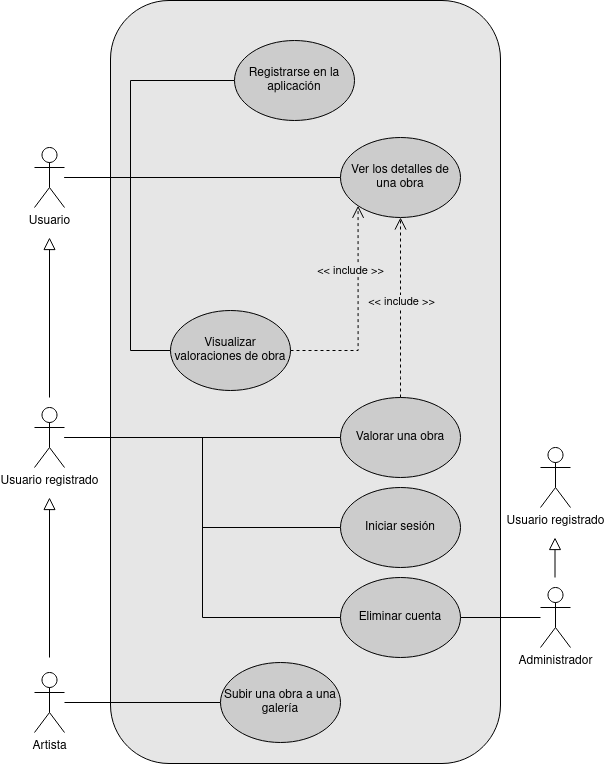
\includegraphics[width=\textwidth]{diagramas/casos_de_uso.png}
    \caption{Diagrama de casos de uso}
    \label{fig:casos_de_uso}
\end{figure}

\begin{figure}[H]
    \centering
    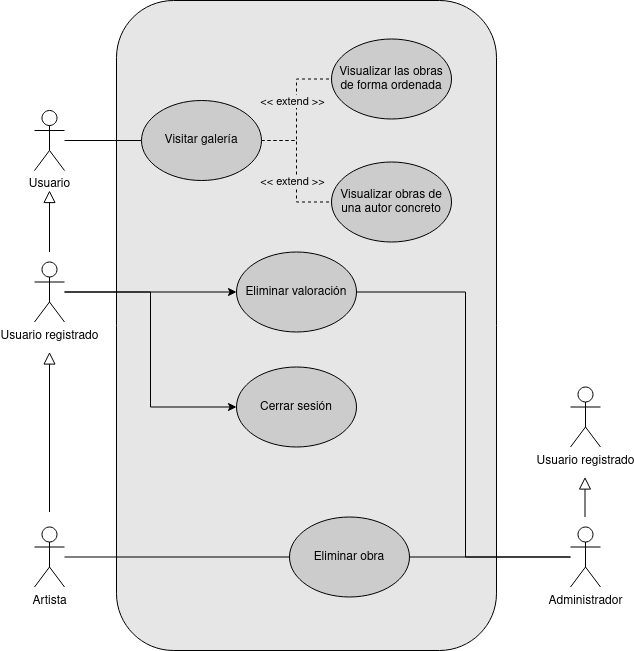
\includegraphics[width=\textwidth]{diagramas/casos_de_uso_2.png}
    \caption{Diagrama de casos de uso (continuación)}
    \label{fig:casos_de_uso_continuacion}
\end{figure}

\newpage
\section{Diagramas de secuencia}
A continuación se van a mostrar los diagramas de secuencia, también realizados
con la herramienta \textit{diagrams.net} \cite{diagramsnet}:

\begin{figure}[H]
    \centering
    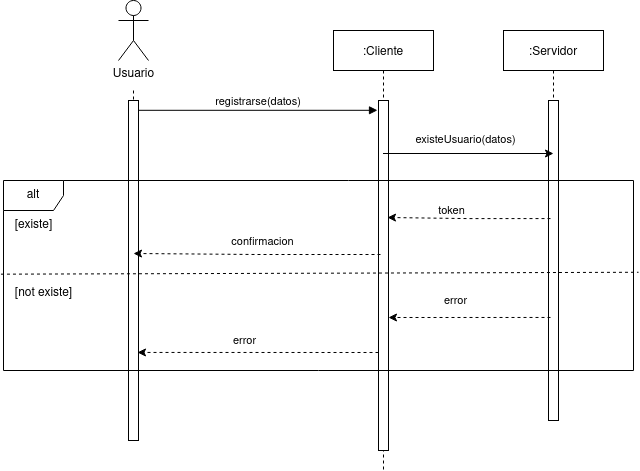
\includegraphics[width=\textwidth]{diagramas/secuencia_registrarse.png}
    \caption{Diagrama de secuencia de registrarse}
    \label{fig:registrarse}
\end{figure}

\begin{figure}[H]
    \centering
    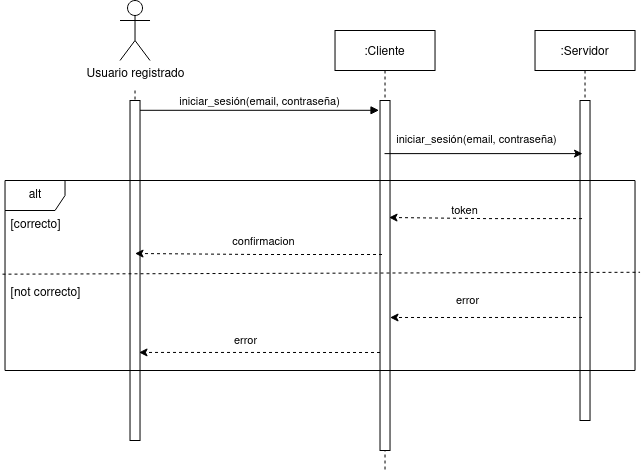
\includegraphics[width=\textwidth]{diagramas/secuencia_iniciar_sesion.png}
    \caption{Diagrama de secuencia de iniciar sesión}
    \label{fig:iniciar_sesion}
\end{figure}

\begin{figure}[H]
    \centering
    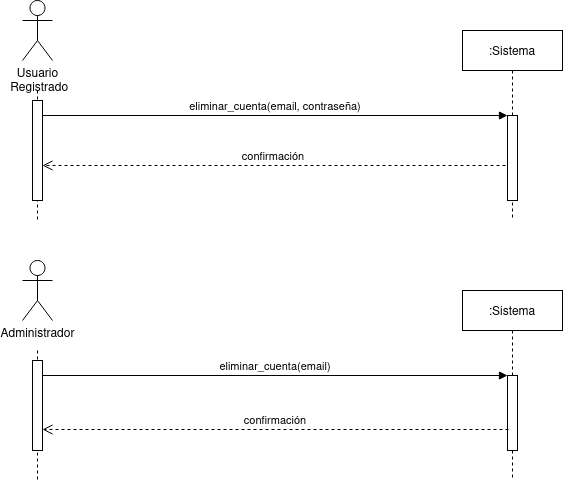
\includegraphics[width=\textwidth]{diagramas/secuencia_eliminar_cuenta.png}
    \caption{Diagrama de secuencia de eliminar cuenta}
    \label{fig:eliminar_cuenta}
\end{figure}

\begin{figure}[H]
    \centering
    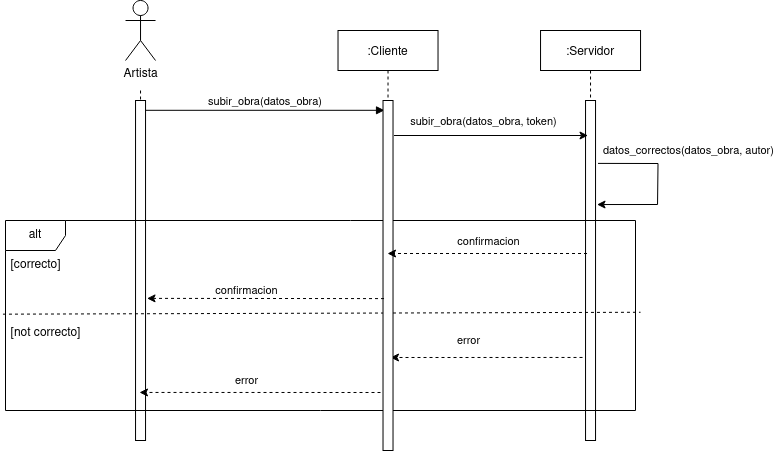
\includegraphics[width=\textwidth]{diagramas/secuencia_subir_obra.png}
    \caption{Diagrama de secuencia de subir obra}
    \label{fig:subir_obra}
\end{figure}

\begin{figure}[H]
    \centering
    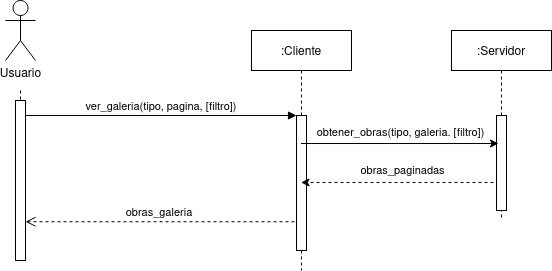
\includegraphics[width=\textwidth]{diagramas/secuencia_mostrar_galeria.png}
    \caption{Diagrama de secuencia de mostrar galería}
    \label{fig:mostrar_galeria}
\end{figure}

\begin{figure}[H]
    \centering
    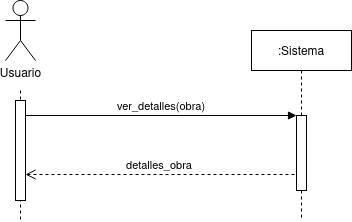
\includegraphics[width=\textwidth]{diagramas/secuencia_mostrar_detalles_obra.png}
    \caption{Diagrama de secuencia de mostrar detalles de obra}
    \label{fig:mostrar_detalles_obra}
\end{figure}

\begin{figure}[H]
    \centering
    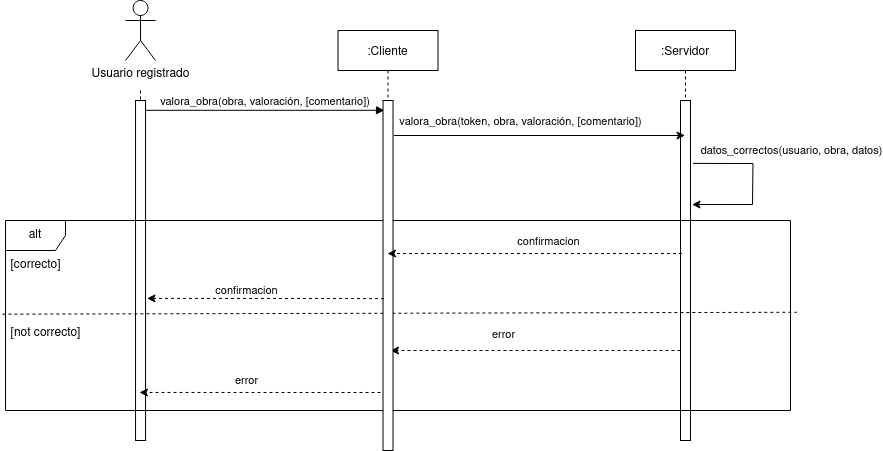
\includegraphics[width=\textwidth]{diagramas/secuencia_valorar_obra.png}
    \caption{Diagrama de secuencia de valorar obra}
    \label{fig:valorar_obra}
\end{figure}

	
	\chapter{Diseño}
En este capítulo se abordará el diseño del sistema. Para ello, en primer
lugar, se va a realizar el diseño de la base de datos con el modelo
entidad-relación, el paso a tablas y la normalización. En segundo lugar,
se realizará el diseño de las interfaces de usuario. Por se hablará del
diseño de la arquitectura del sistema.

\section{Diseño de base de datos}
En esta sección vamos a abordar el diseño de la base de datos.
Comenzaremos con el modelo entidad-relación y terminaremos con el paso a
tablas y la normalización.

\subsection{Modelo Entidad-Relación}
En nuestro caso, la base de datos va a estar formada por las siguientes
entidades:

\begin{itemize}
    \item \textbf{Usuario}: Esta entidad representa a los usuarios de la aplicación.
    \item \textbf{Artista}: Esta entidad representa a los artistas de la aplicación.
    \item \textbf{ObraDeArte}: Esta entidad representa a las obras de arte de la aplicación.
    \item \textbf{Valoración}: Esta entidad representa a las valoraciones de las obras de
    arte que realizan los usuarios.
\end{itemize}

En la figura \ref{fig:e-r} se muestra el modelo entidad-relación de la base de
datos. En dicho modelo se encuentran las entidades con sus atributos y las
relaciones entre ellas.

Vemos que la entidad \texttt{Artista} hereda de la entidad \texttt{Usuario}.
Esto se hace para poder relacionar la entidad \texttt{Artista} con la entidad
\texttt{ObraDeArte} a través de la relación \texttt{Tiene} y que sea independiente
de la entidad \texttt{Usuario} ya que solamente los usuarios que sean artistas
podrán tener obras de arte.

La entidad \texttt{Usuario} tiene una relación \texttt{Realiza} con la entidad
\texttt{Valoración} indicando que un usuario puede realizar varias valoraciones.
A su vez la entidad \texttt{Valoración} tiene una relación \texttt{Pertenece} con
la entidad \texttt{ObraDeArte} indicando que una valoración pertenece a una obra
de arte.

\begin{figure}[H]
  \centering
  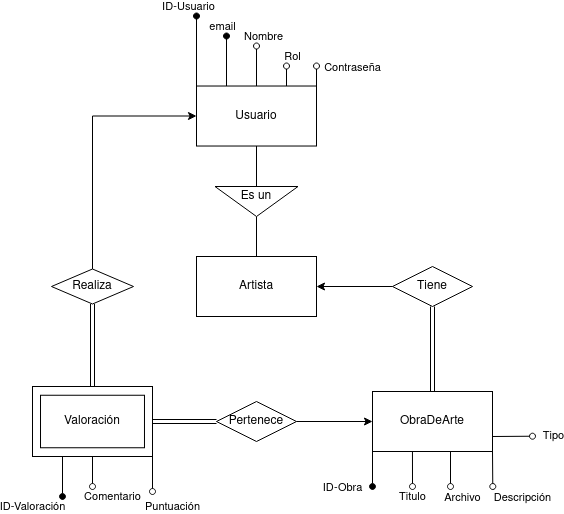
\includegraphics[width=\textwidth]{diagramas/e-r}
  \caption{Modelo entidad-relación}
  \label{fig:e-r}
\end{figure}

\subsection{Paso a tablas}
A continuación vamos a realizar el paso a tablas del modelo entidad-relación. Para
ello haremos las tablas primero de las entidades fuertes, luego entidades débiles
y por último las relaciones.

\begin{enumerate}
    \item \[ \texttt{Usuario}(\underline{ID-Usuario}_{CP}, \underline{Email}_{CC}, Nombre, Contraseña) \]
    \item \[ \texttt{Artista}(\underline{ID-Usuario}_{CP}^{CE1}) \]
    \item \[ \texttt{ObraDeArte}(\underline{ID-Obra}_{CP}, Titulo, Descripción, Tipo, Archivo) \]
    \item \[ \texttt{Valoración}(\underline{ID-Valoración}_{CP}, Puntuación, Comentario) \]
    \item \[ \texttt{Tiene}(\underline{ID-Obra}_{CP}^{CE3}, ID-Usuario^{CE2}) \]
    \item \[ \texttt{Pertenece}(\underline{ID-Valoración}_{CP}^{CE4}, ID-Obra^{CE3}) \]
    \item \[ \texttt{Realiza}(\underline{ID-Valoración}_{CP}^{CE4}, ID-Usuario^{CE1}) \]
\end{enumerate}

\vspace{1cm}
Ahora se va a proceder a fusionar las tablas que sean posibles. Además,
dado que la tabla \texttt{Artista} no tiene atributos propios y solamente tiene
una clave externa que es clave primaria en la tabla \texttt{Usuario} (que es la
tabla padre), se puede fusionar con dicha tabla, añadiendo a esta una columna
que indique si el usuario es artista o no, será el atributo \texttt{Rol}.

\begin{enumerate}
    \item \[ \texttt{Usuario}(\underline{ID-Usuario}_{CP}, \underline{Email}_{CC}, Nombre, Contraseña, Rol) \]
    \item \[ \texttt{ObraDeArte}(\underline{ID-Obra}_{CP}, Titulo, Descripción, Tipo, Archivo, ID-Usuario^{CE1}) \]
    \item \[ \texttt{Valoración}(\underline{ID-Valoración}_{CP}, Puntuación, Comentario, ID-Obra^{CE2}, ID-Usuario^{CE1}) \]
\end{enumerate}

\subsection{Normalización}
Dado que todos los atributos de las tablas están en 1FN, vamos a proceder a
normalizar las tablas a 2FN y 3FN.

\subsubsection{2FN}
Para que una tabla esté en 2FN debe estar en 1FN y además todos los atributos
que no pertenezcan a la clave primaria deben depender de esta.

En nuestro caso, todas las tablas están en 1FN y además todos los atributos
dependen de la clave primaria, por lo que todas las tablas están en 2FN.

\subsubsection{3FN}
Para que una tabla esté en 3FN debe estar en 2FN y además todos los atributos
que no pertenezcan a la clave primaria deben depender únicamente de dicha
clave primaria y no de otros atributos.

En nuestro caso, todas las tablas están en 2FN y además todos los atributos
dependen de la clave primaria y no de otros atributos no-clave, por lo que
todas las tablas están en 3FN.

\section{Diseño de interfaces de usuario}

\section{Diseño de la arquitectura del sistema}
A continuación se va a explicar la arquitecura del sistema utilizada.
Para la creación de la aplicación web se va a utilizar el patrón
Modelo-Vista-Controlador (MVC).

\subsection{Modelo-Vista-Controlador}
Este patrón de arquitectura se basa, como se explica en este artículo \cite{mvc},
en separar la lógica de la aplicación en tres partes:

\begin{itemize}
    \item \textbf{Modelo}: El modelo representa la información con la que trabaja
    la aplicación. En el caso de la aplicación que vamos a desarrollar, el modelo
    será la base de datos y las funciones del backend que se encarguen de gestionarla.
    \item \textbf{Vista}: La vista es la parte encargada de mostrar la información
    al usuario y permitir que este interactúe con la aplicación. En el caso de la
    aplicación que vamos a desarrollar, la vista será la parte del frontend.
    \item \textbf{Controlador}: El controlador es el encargado de gestionar las
    peticiones del usuario y realizar las acciones correspondientes. Es el enlace
    entre la vista y el modelo. En nuestra aplicación el controlador será la parte
    del backend que se encargue de gestionar las peticiones provenientes del frontend
    y a través de una serie de funciones \textit{getters} y \textit{setters} se
    pedirá y modificará la información del modelo.
\end{itemize}

En la figura \ref{fig:mvc} se muestra un diagrama de la arquitectura MVC de la
aplicación.

\begin{figure}[H]
  \centering
  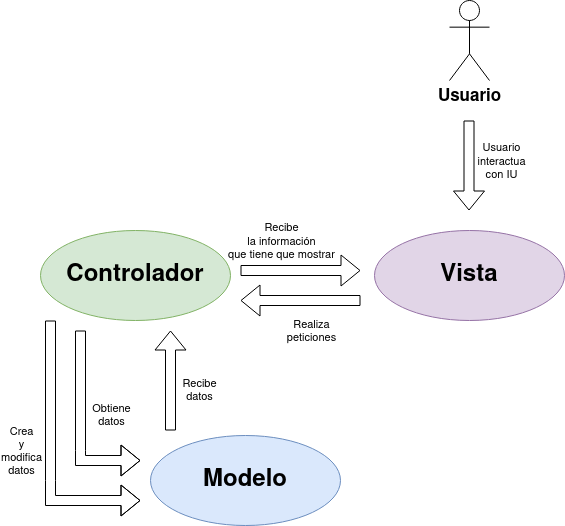
\includegraphics[width=\textwidth]{diagramas/mvc}
  \caption{Modelo-Vista-Controlador}
  \label{fig:mvc}
\end{figure}


	% Desarrollo bajo sprints: 
	% 	1. Permitir registros y login de usuarios
	% 	2. Desarrollo del sistema de incidencias
	% 	3. Desarrollo del sistema de denuncias administrativas y accidentes
	% 	4. Desarrollo del sistema de croquis
	%   5. Instalación de la aplicación de manera automática
	\chapter{Implementación}
En este capítulo se va a abordar la implementación del sistema. Para ello, en
primer lugar, se van a explicar las herramientas y tecnologías que se han utilizado
y el porqué de su elección. En segundo lugar, se explicará la implementación de la
base de datos, se mostrará el diagrama de clases y, por último, se explicará la
implementación de la aplicación, tanto del backend como del frontend.

\section{Herramientas y tecnologías}
En este apartado se van a explicar las herramientas y tecnologías utilizadas
para el desarrollo de la aplicación.

\subsection{Control de versiones}
Para realizar un seguimiento del desarrollo de la aplicación se ha utilizado la
herramienta de control de versiones \textit{Git} \cite{git}, que permite llevar un
control de los cambios realizados en el código fuente de la aplicación. Además, estos
cambios se han ido subiendo a la plataforma \textit{GitHub} \cite{github}.

Para seguir una estructura de los commits que se van realizando, se han ido escribiendo
los mensajes de commit con el formato "\texttt{<stack>} - \texttt{<mensaje>}", donde
\texttt{<stack>} es \textit{SERVER} o \textit{CLIENT} dependiendo de si el commit afecta
al backend o al frontend de la aplicación, y \texttt{<mensaje>} es la descripción de los
cambios que se han realizado.

En la figura \ref{fig:commits} se puede ver un ejemplo de una captura sacada
del listado de commits realizados en el repositorio de \textit{GitHub} \cite{github}.

\begin{figure}[H]
  \centering
  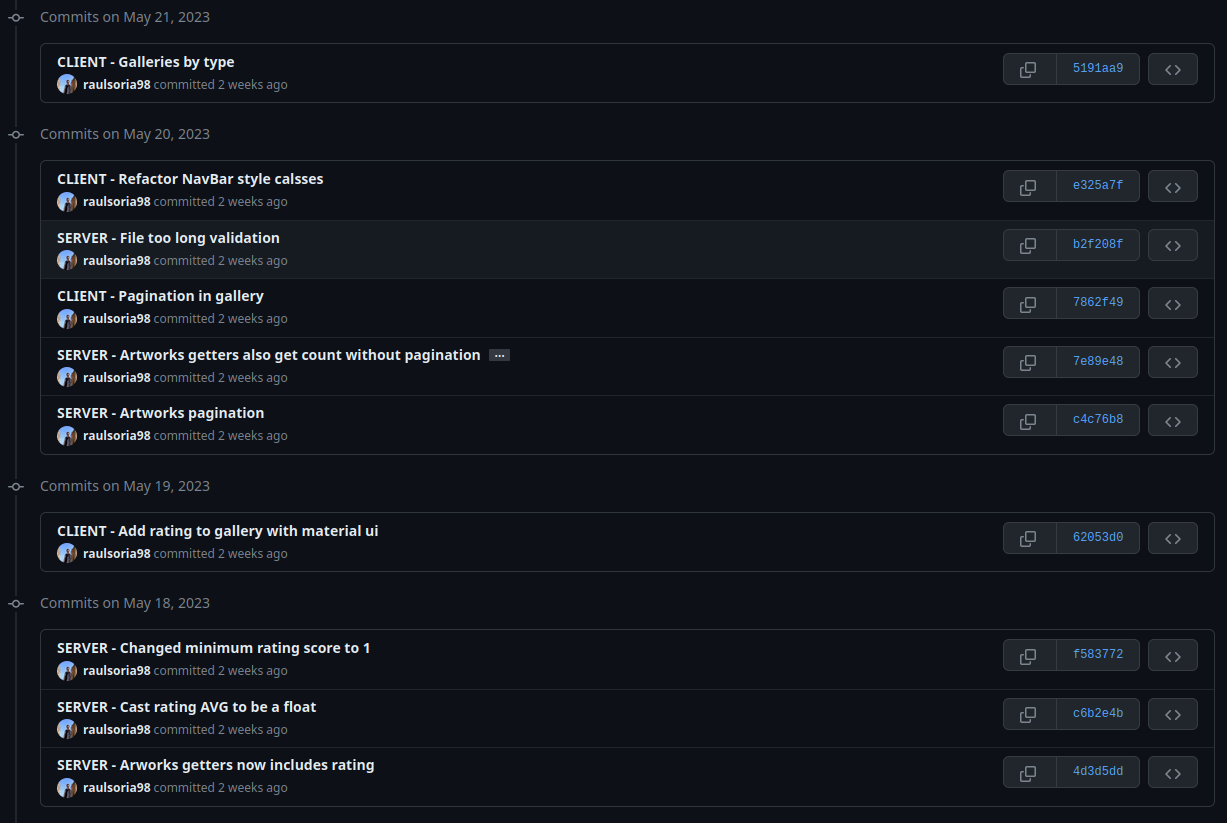
\includegraphics[width=1\textwidth]{commits}
  \caption{Ejemplo de mensajes de commit}
  \label{fig:commits}
\end{figure}

\subsection{Base de datos}
Para la base de datos había que elegir en primer lugar entre una base de datos
relacional o una base de datos no relacional.

En este artículo \cite{relational-vs-non-relational} se explica la diferencia entre
un tipo de base de datos y otro, las ventajas que tiene cada una y en qué casos es
más recomendable utilizar una u otra.

En el caso de nuestra aplicación, se ha optado por utilizar una base de datos relacional
ya que, aunque la base de datos no va a ser muy grande, sí que va a tener una estructura
bien definida con relaciones fuertes entre las tablas.

También es necesario elegir el gestor de base de datos que se va a utilizar, ya que
existen varios gestores de bases de datos relacionales. En nuestro caso se ha optado
por utilizar \textit{MySQL} \cite{mysql} ya que es el gestor de bases de datos
relacionales más utilizado y es el que más conozco personalmente.

\subsection{Backend}
Para el desarrollo del backend de la aplicación se ha utilizado \textit{Node.js}
\cite{nodejs} que es un entorno de ejecución de JavaScript. Se ha elegido este
entorno porque quería aprender a utilizarlo dada su popularidad y porque así podría
utilizar JavaScript tanto en el backend como en el frontend. Este último punto
hizo que descartara utilizar otros frameworks como \textit{Django} \cite{django}
o \textit{Ruby on Rails} \cite{ruby-on-rails}.

Como framework complementario a \textit{Node.js} se ha utilizado \textit{Express}
\cite{express} que facilita la creación de aplicaciones web y de APIs en \textit{Node.js}.

\subsection{Frontend}
Para el desarrollo del frontend de la aplicación se barajaron varias opciones.
En primer lugar, se pensó en utilizar \textit{Angular} \cite{angular} ya que es un
framework bastante popular y con el que ya había trabajado anteriormente. Sin embargo,
se descartó esta opción porque, como explican en este artículo \cite{angular-vs-react},
este es un framework muy completo y pensado para aplicaciones grandes donde prima el
trabajo en equipo ya que su estructura es fija y esto la hace más compleja. Mientras
que \textit{React} \cite{react} es una biblioteca más sencilla y flexible que permite
crear aplicaciones pequeñas como la nuestra de manera sencilla y sin una gran curva de
aprendizaje.

También se barajó la opción de utilizar \textit{Vue.js} \cite{vuejs} ya que es una
librería de la que también había oído hablar y que también usa JavaScript.
Como comentan en este otro artículo \cite{vuejs-vs-react}, \textit{Vue.js} \cite{vuejs}
también es una librería bastante sencilla y ligera, cuyos módulos se pueden ir añadiendo
según se vayan necesitando. Sin embargo, se descartó esta opción porque, aunque
\textit{Vue.js} \cite{vuejs} es más sencillo que \textit{React} \cite{react}, este
último tiene mayor rendimiento, además, me llamaba más la atención y quería aprender a
utilizarlo.


\section{Implementación de la base de datos}
Para la implementación de la base de datos \textit{MySQL} \cite{mysql} se ha utilizado
\textit{Sequelize} \cite{sequelize} que es un ORM (Object-Relational Mapping) para
\textit{Node.js} \cite{nodejs} que permite trabajar con bases de datos relacionales
como la que se ha utilizado en este proyecto.

Tal y como se explica en este artículo \cite{orm}, \textit{'Un ORM (Object Relational
Mapping o Mapeo Objeto-Relacional en castellano) es una herramienta que nos permite mapear, o lo
que es lo mismo, convertir los objetos de tu aplicación a un formato adecuado para ser
almacenados en cualquier base de datos, creándo para ello una base de datos virtual
donde los datos disponibles en nuestra aplicación quedan vinculados con la base de datos
final.'}

Con \textit{Sequelize} \cite{sequelize} se define la conexión a la base de datos como se
puede ver en el código de la imágen \ref{fig:sequelize-db} correspondiente al archivo
\texttt{config/db.js}. Creando un objeto \texttt{sequelize} que servirá para,
posteriormente, realizar la conexión o definir los modelos de la base de datos. Como se
puede ver, el nombre de la base de datos, el usuario, la contraseña, el host y el puerto
se han definido en variables de entorno en un archivo \texttt{.env} para que no se vean
reflejados en el código fuente y así evitar que se suban a \textit{GitHub} \cite{github}.

\begin{figure}[H]
  \centering
  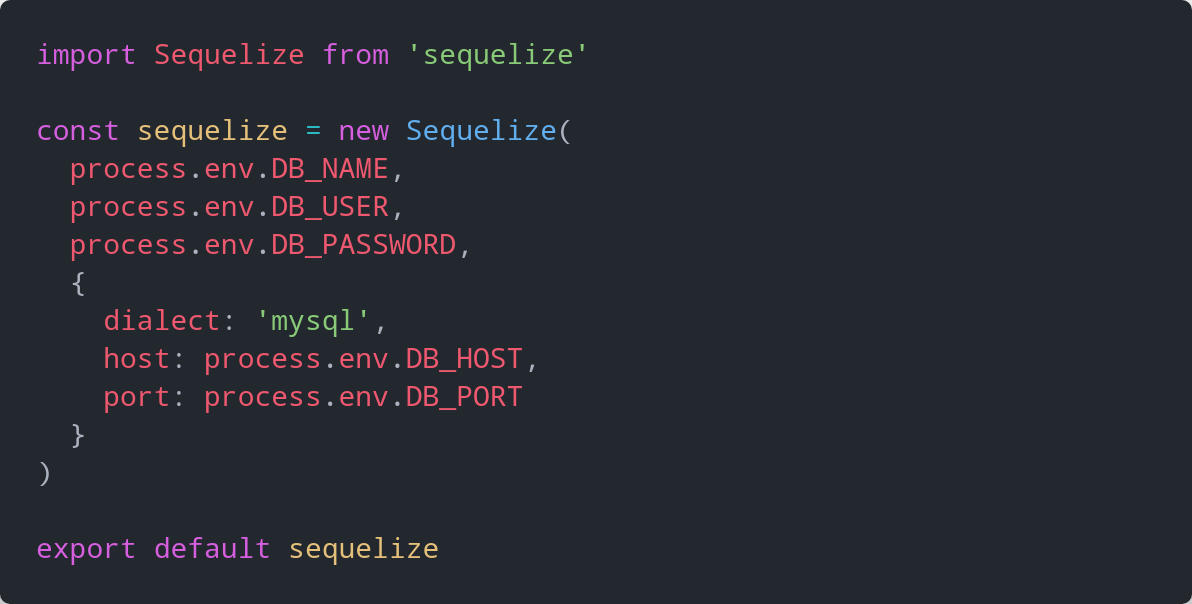
\includegraphics[width=1\textwidth]{img/sequelize-db}
  \caption{Definición de la conexión a la base de datos con \textit{Sequelize}}
  \label{fig:sequelize-db}
\end{figure}

Una vez definida la conexión a la base de datos, se realiza la conexión con la misma
mediante el método \texttt{authenticate()} como se puede ver en el código de la imágen
\ref{fig:sequelize-connect} donde se define una función de conexión que se ejecuta
cuando se inicia la aplicación.

\begin{figure}[H]
  \centering
  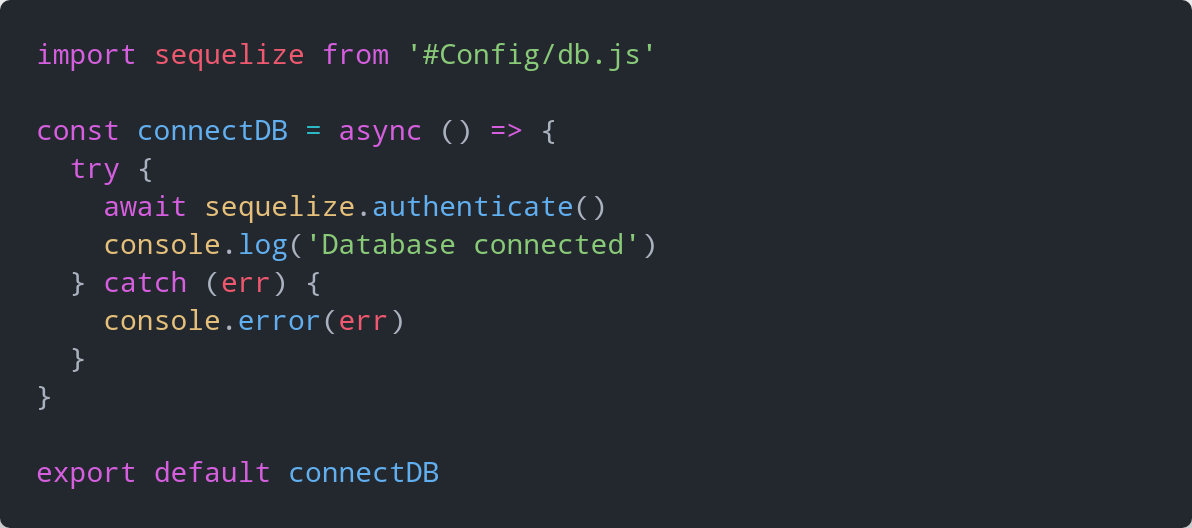
\includegraphics[width=1\textwidth]{img/sequelize-connect}
  \caption{Conexión a la base de datos con \textit{Sequelize}}
  \label{fig:sequelize-connect}
\end{figure}

Para la definición de los modelos de la base de datos se ha seguido la documentación
de \textit{Sequelize} \cite{sequelize-models} donde se explica cómo definir los modelos.
En la aplicación se han creado los archivos correspondientes
a cada modelo. Como por ejemplo el archivo \texttt{artwork.js}, cuyo código se puede ver
en la imágen \ref{fig:artwork-model}, donde se define el modelo \texttt{Artwork} con sus
atributos, validaciones y constraints.

\begin{figure}[H]
  \centering
  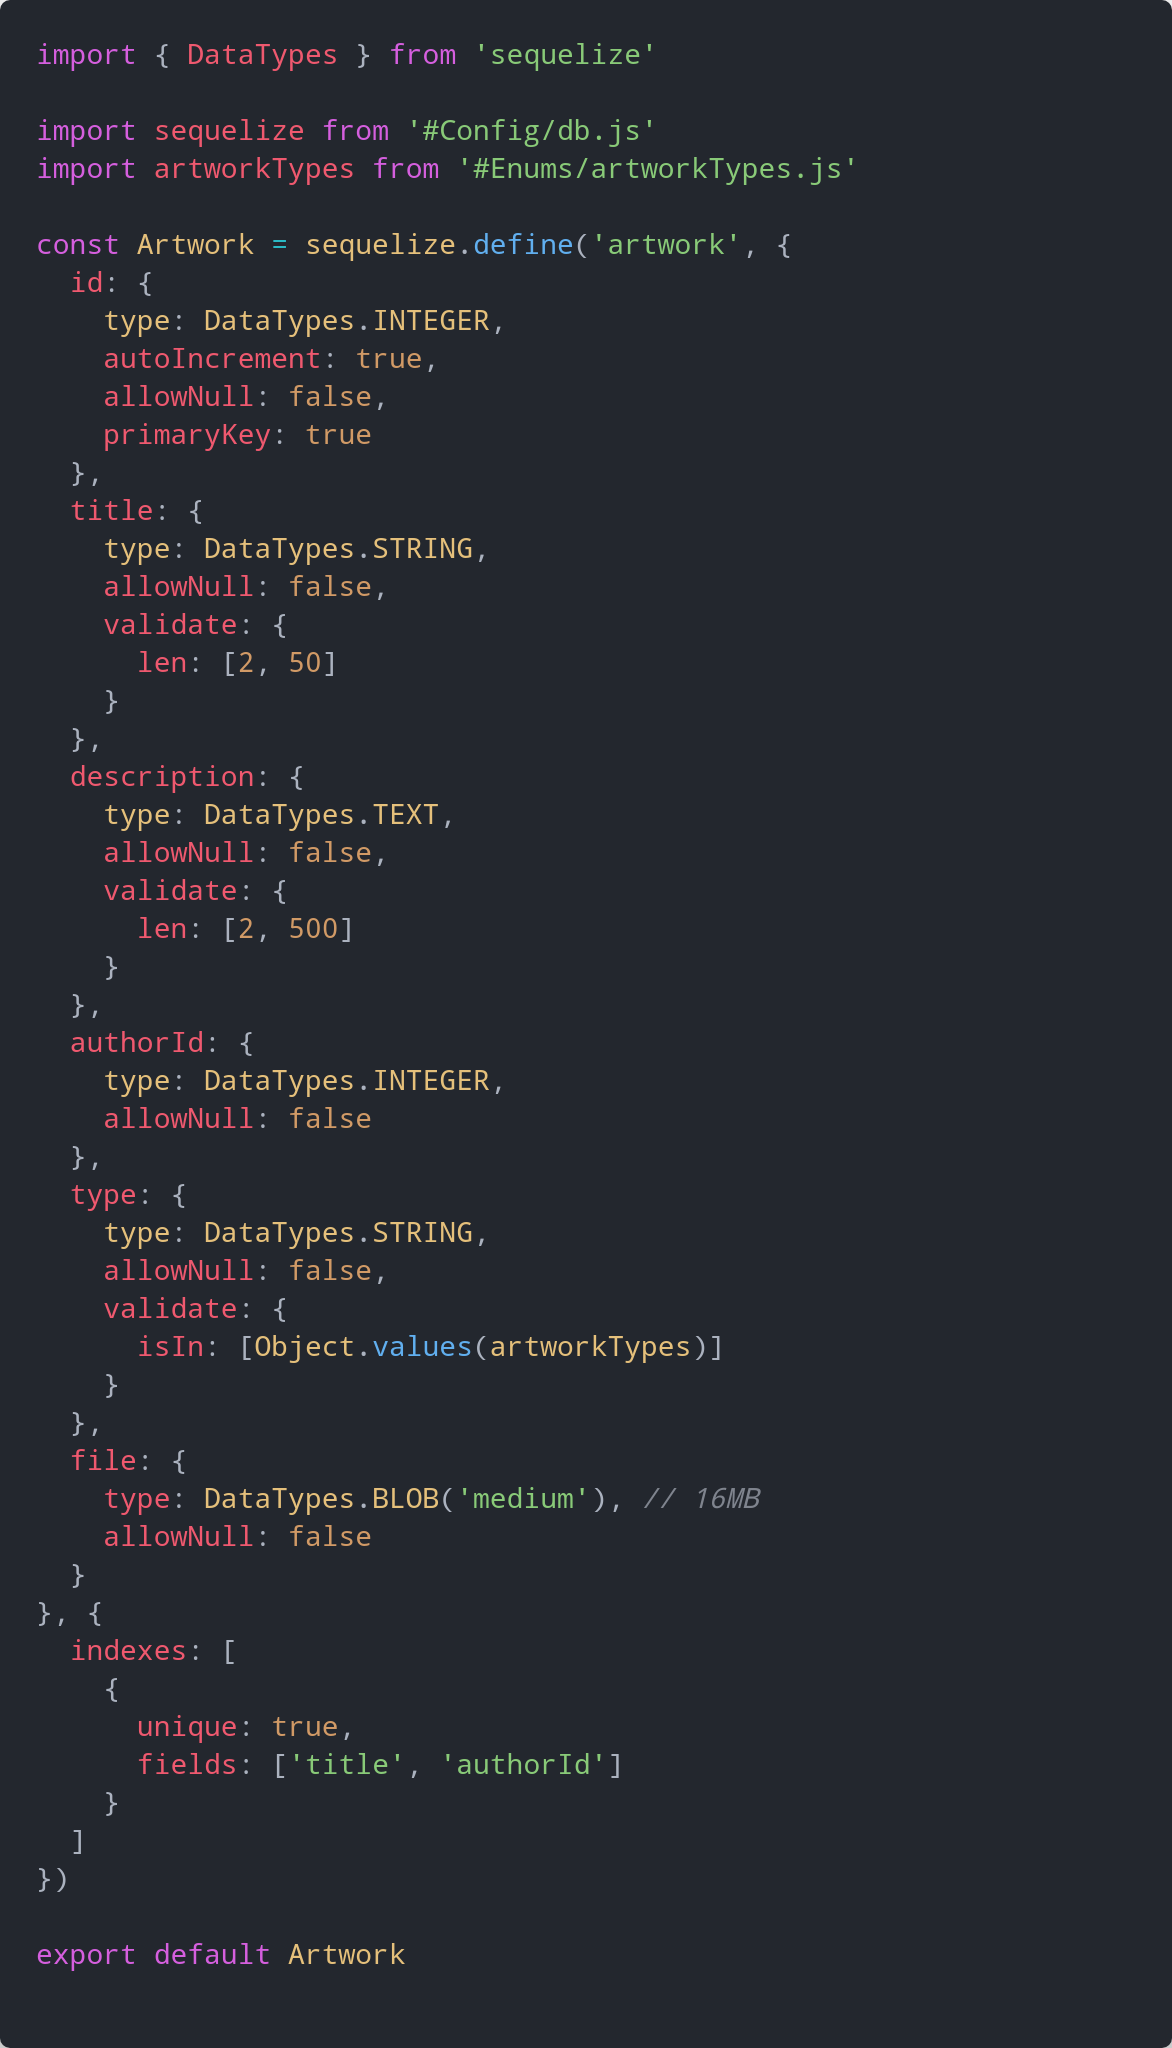
\includegraphics[width=0.8\textwidth]{img/artwork-model}
  \caption{Definición del modelo \texttt{Artwork}}
  \label{fig:artwork-model}
\end{figure}

Para las relaciones entre los distintos modelos se han seguido las instrucciones
de la documentación oficial \cite{sequelize-associations}. Se definen en una función
\texttt{associateModels} que se ejecuta justo después de realizar la conexión a la base
de datos. Como se puede ver en el código de la imágen \ref{fig:associate-models}, se
define la relación uno a muchos entre el modelo \texttt{User} y el modelo \texttt{Artwork},
la relación uno a muchos entre el modelo \texttt{User} y el modelo \texttt{Rating} y la
relación uno a muchos también, entre el modelo \texttt{Artwork} y el modelo \texttt{Rating}.

También se puede ver que se definen las claves externas de cada relación y un alias para
cada una de ellas. Esto permite realizar consultas que incluyan datos de los modelos
relacionados de manera más sencilla.

\begin{figure}[H]
  \centering
  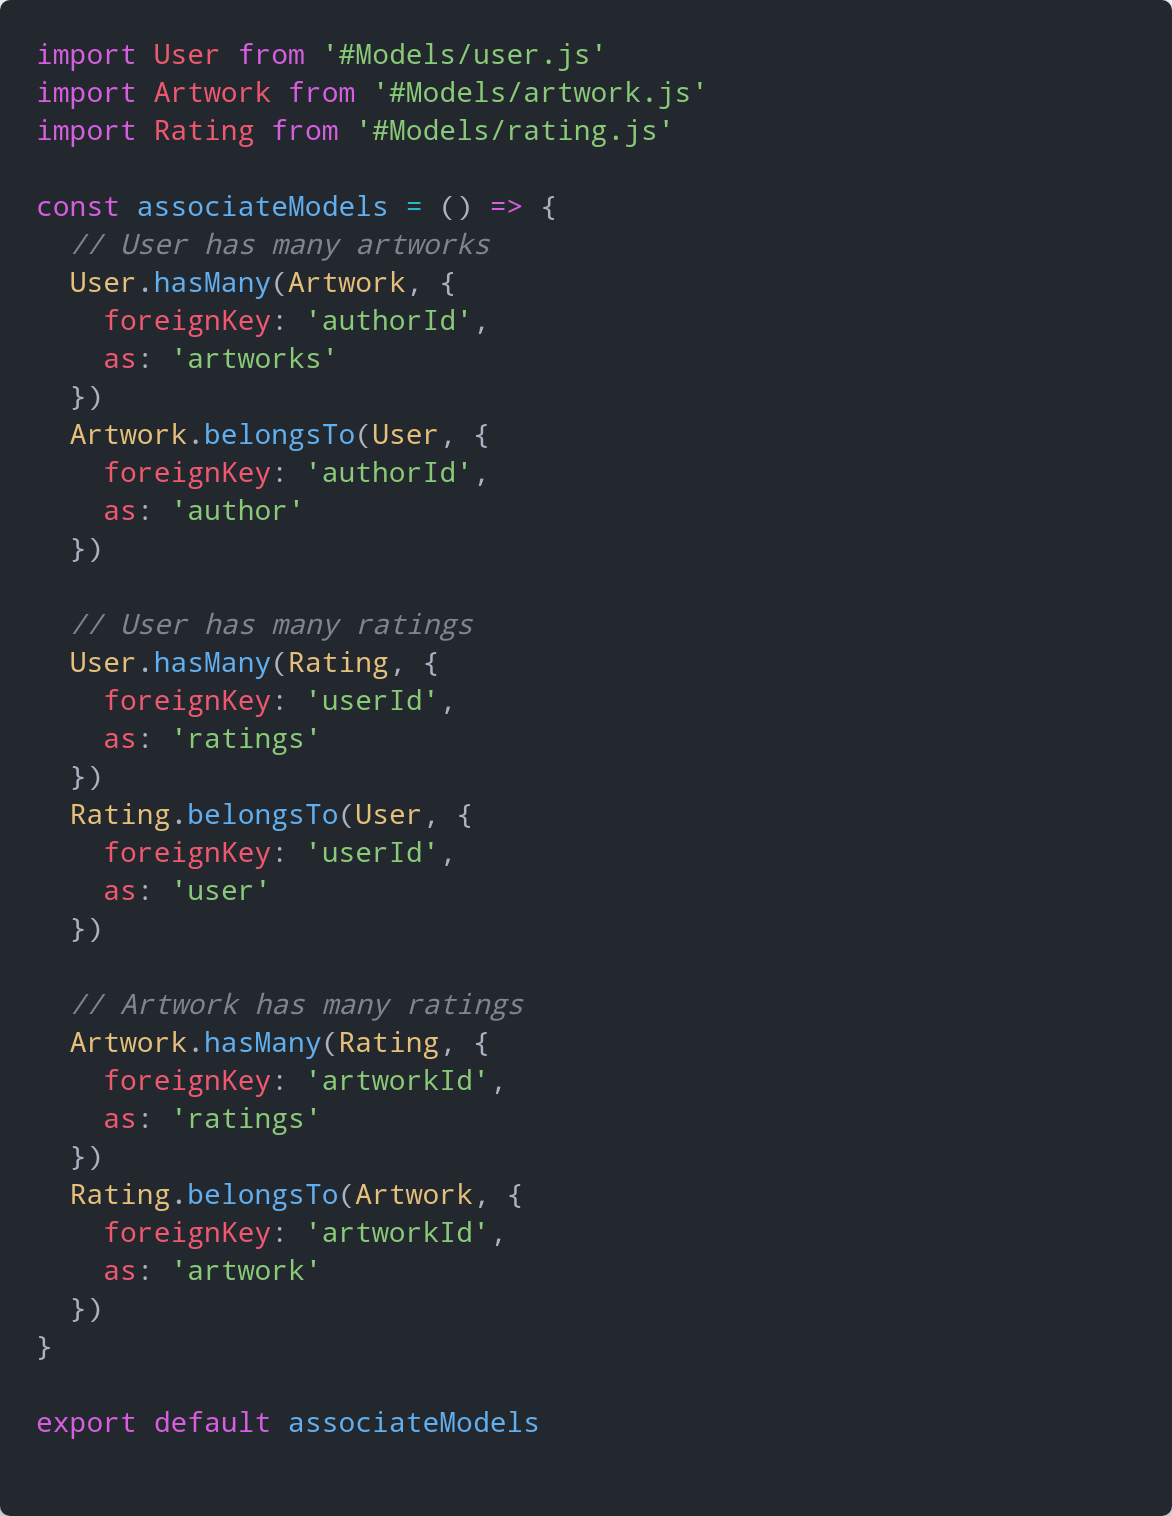
\includegraphics[width=1\textwidth]{img/associate-models}
  \caption{Definición de las relaciones entre los modelos}
  \label{fig:associate-models}
\end{figure}

Para la gestión de la base de datos se ha utilizado \textit{PhpMyAdmin} \cite{phpmyadmin}
que es una herramienta de administración de bases de datos basada en web, ofreciendo una
interfaz gráfica desde la que poder ver y gestionar los datos de la aplicación por parte
de los administradores.

Todas las contraseñas almacenadas en la base de datos se han encriptado utilizando
la librería \textit{bcrypt} \cite{bcrypt-nodejs} de \textit{Node.js} \cite{nodejs} que usa
la función de hashing \textit{bcrypt} \cite{bcrypt} basada en el cifrado Blowfish que
permite encriptar contraseñas de manera segura.

\newpage

\section{Diagrama de clases}
A continuación, en la figura \ref{fig:class-diagram}, se observa el diagrama de clases
de la aplicación. En él se pueden ver las tres clases de la aplicación: \texttt{users},
\texttt{artworks} y \texttt{ratings}. En ellas se ven sus atributos y las relaciones
entre ellas.

Como se puede ver, la clase \texttt{users} tiene una relación uno a muchos
con la clase \texttt{artworks} y la clase \texttt{ratings} tiene una relación muchos a
uno con las clases \texttt{users} y \texttt{artworks}.

\begin{figure}[H]
  \centering
  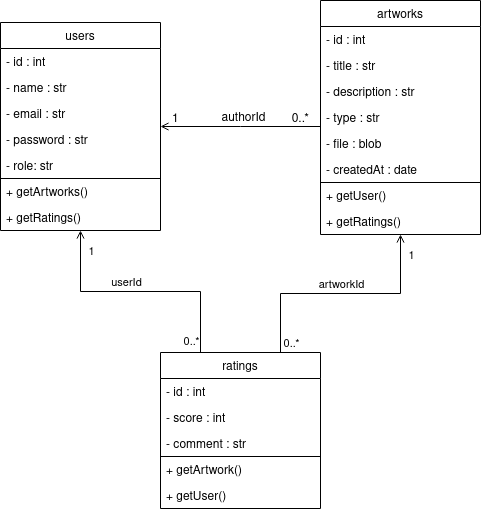
\includegraphics[width=0.9\textwidth]{diagramas/diagrama_clases}
  \caption{Diagrama de clases}
  \label{fig:class-diagram}
\end{figure}

\newpage

\section{Implementación de la aplicación}
A continuación se van a explicar los puntos más importantes de la implementación de la
aplicación, tanto en el backend como en el frontend.

\subsection{Backend}
El backend de la aplicación se ha desarrollado utilizando \textit{Node.js} \cite{nodejs}
y \textit{Express} \cite{express}. Para crear el servidor de la aplicación se ha creado
la aplicación de \textit{Express} como se muestra en el código de la imágen
\ref{fig:express-app}.

\begin{figure}[H]
  \centering
  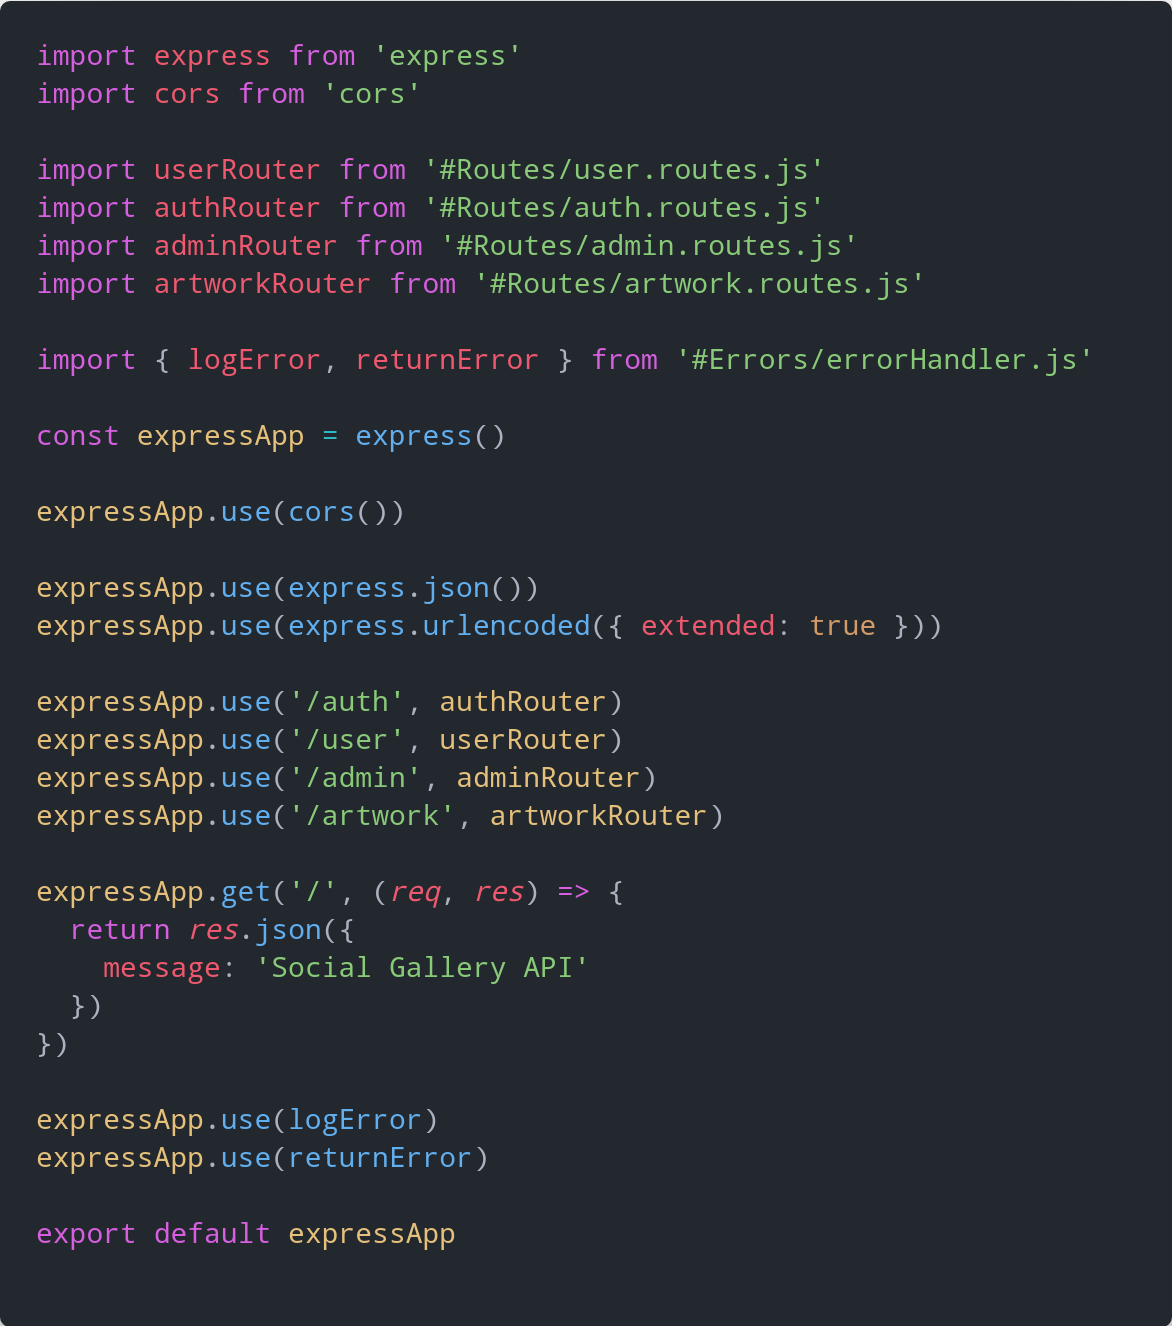
\includegraphics[width=\textwidth]{img/express-app}
  \caption{Creación de la aplicación de \textit{Express}}
  \label{fig:express-app}
\end{figure}

En él se define en primer lugar la aplicación de \textit{Express} y se le añaden los
middlewares necesarios, comenzando con el middleware \texttt{cors} \cite{express-cors}
que permite que se puedan realizar peticiones a la API desde el frontend.

A continuación se añade el middleware \texttt{express.json()} \cite{express-json}
para que la aplicación pueda recibir datos en formato \texttt{JSON}.
Después se añade el middleware de \texttt{express.urlencoded({ extended: true })}
\cite{express-urlencoded} para que la aplicación pueda recibir datos en formato
\texttt{string} o \texttt{array}.

Después se añaden los routers de la aplicación \cite{express-router} que se encargan
de gestionar las rutas de la API y llamar a las funciones correspondientes de los
controladores. También se añade la ruta por defecto que devuelve un mensaje con el
nombre de la API.

Por último, se añaden un par de middlewares más para gestionar los errores que se
puedan producir en la aplicación. Uno se encarga de mostrarlos por consola y el otro
de devolverlos en formato \texttt{JSON} y con su código de error correspondiente.

\subsubsection{Rutas}
Como se ha comentado anteriormente, los routers se encargan de gestionar las rutas
de la API y llamar a las funciones correspondientes de los controladores. Son
middlewares que agrupan rutas que tienen algo en común. En este caso, se han creado
routers para agrupar las rutas de autenticación, de los usuarios, las obras de arte
y las rutas que son para los administradores.

Como ejemplo, se puede ver el código del router de autenticación en la imágen
\ref{fig:auth-router}. En él se definen las rutas de autenticación, que son las de
inicio de sesión y registro, ambas peticiones son de tipo \texttt{POST} \cite{post-request}.
El primer parámetro que se le pasa a la función \texttt{post} de \textit{Express}
es el \texttt{path} o ruta de la petición, como se explica en la documentación
\cite{express-router}. Los siguientes parámetros son los diferentes middlewares que
se van a ejecutar para esa ruta. En este caso, ambas rutas ejecutan en primer lugar
un middleware de validación de los datos que llegan con la petición (estos middlewares
se explicarán más adelante, en la sección \ref{sssec:DTOs}). A continuación, se ejecuta
la función del controlador de autenticación correspondiente a la ruta.

\begin{figure}[H]
  \centering
  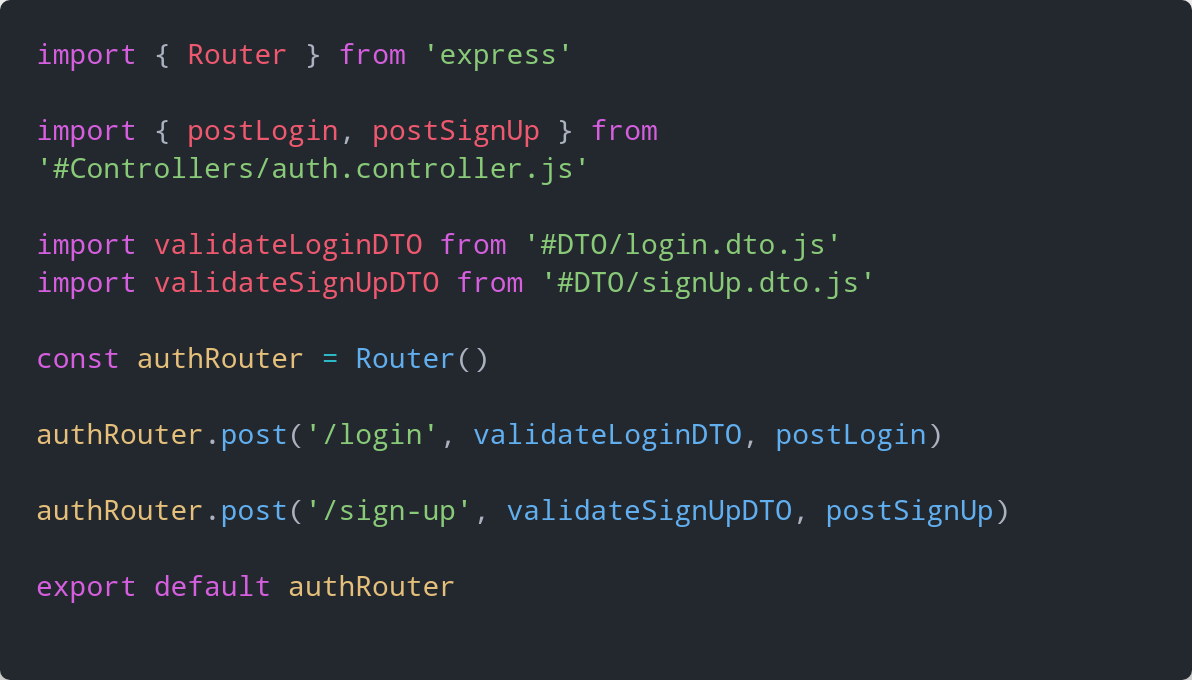
\includegraphics[width=1\textwidth]{img/auth-router}
  \caption{Router de autenticación}
  \label{fig:auth-router}
\end{figure}

\subsubsection{Controladores}
Los controladores son los encargados de realizar las funciones que se ejecutan al
realizar una petición a la API. En el caso de esta aplicación, se han creado
controladores para la autenticación, los usuarios, las obras de arte y los administradores,
cada uno con sus funciones correspondientes. Estas funciones son en realidad middlewares
que se encargan de realizar las acciones necesarias para cada petición.

Un middleware es una función que, como se explica en la documentación de \textit{Express}
\cite{express-middleware}, recibe por parámetros tres objetos:

\begin{itemize}
  \item \texttt{req}: objeto de petición (\textit{request}) que contiene la información
  de la petición HTTP.
  \item \texttt{res}: objeto de respuesta (\textit{response}) que contiene la información
  de la respuesta HTTP que se va a enviar.
  \item \texttt{next}: función que, al ejecutarse, ejecuta el siguiente middleware que se
  haya definido para esa ruta, ya que para una ruta se pueden ejecutar varios middlewares.
\end{itemize}

La nomenclatura utilizada para definir los distintos middlewares de los controladores es
la siguiente: \texttt{<tipoRequest><NombreFuncion>}. Donde \texttt{<tipoRequest>} es el
tipo de petición HTTP que se recibe (\texttt{GET}, \texttt{POST}, \texttt{PUT} o
\texttt{DELETE}) y \texttt{<NombreFuncion>} es el nombre de la función. Por ejemplo,
la función que se encarga de realizar el inicio de sesión de un usuario se llama
\texttt{postLogin} ya que es una petición \texttt{POST}. Todo esto se puede ver en la
imágen \ref{fig:auth-controller} donde se muestra el código del controlador de
autenticación.

\begin{figure}[H]
  \centering
  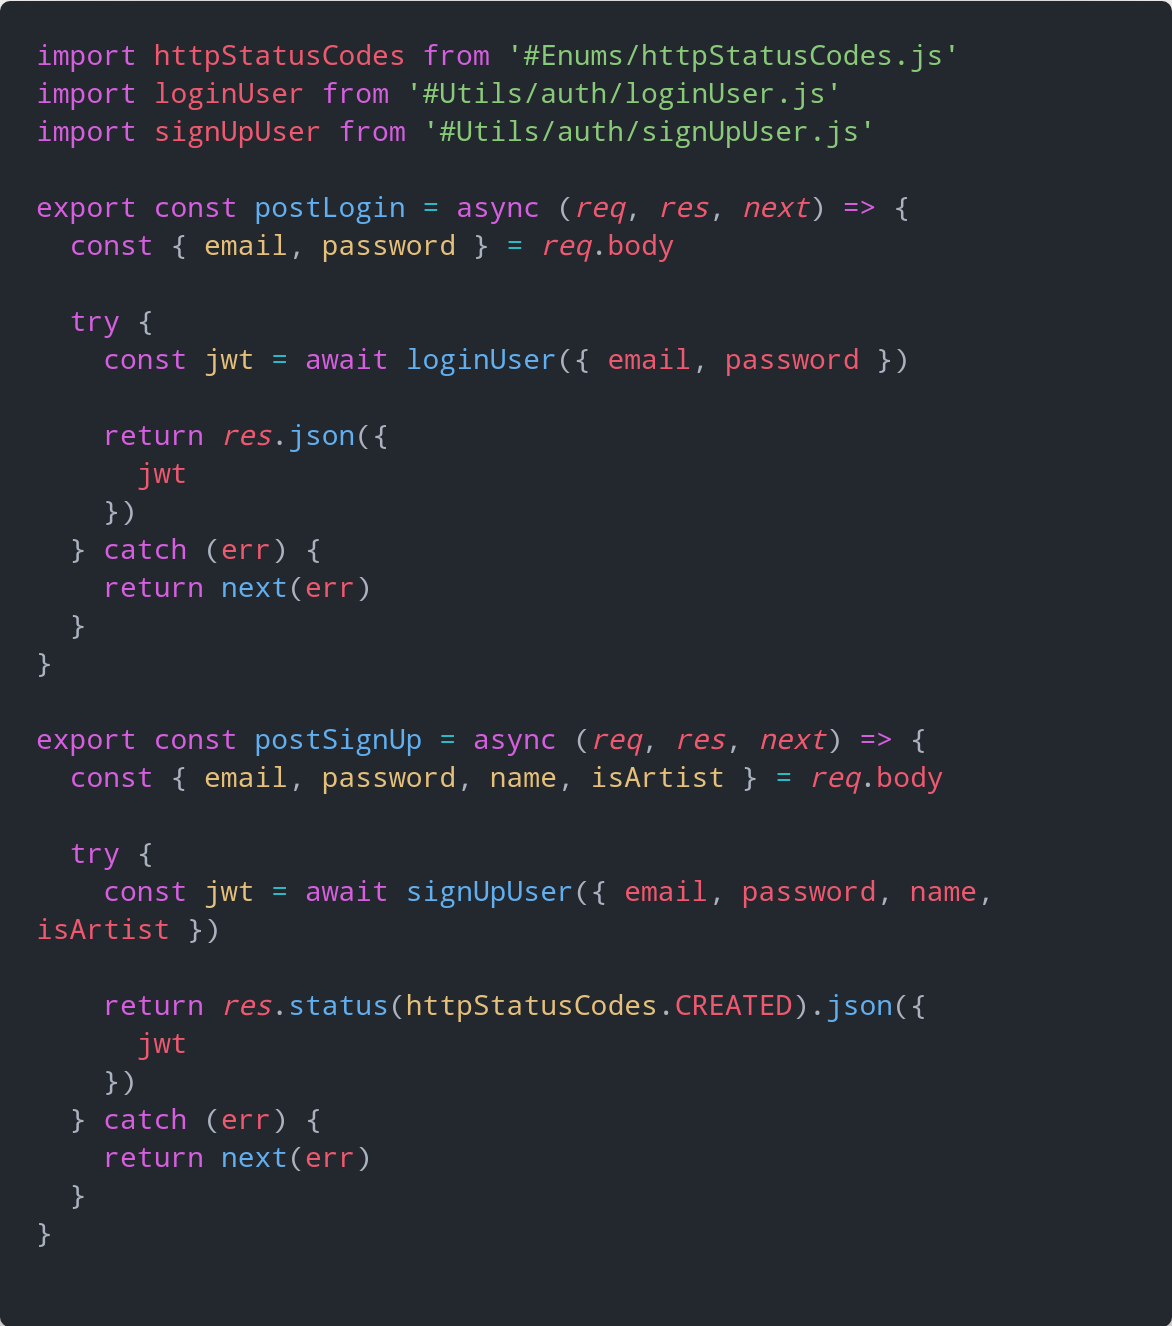
\includegraphics[width=1\textwidth]{img/auth-controller}
  \caption{Controlador de autenticación}
  \label{fig:auth-controller}
\end{figure}

En estas funciones podemos ver cómo en primer lugar se obtienen los datos del body de
la petición y no hace falta comprobar si existen o son correctos ya que de eso se ha
encargado el middleware de DTO (Data Transfer Object), que habíamos mencionado al hablar
de las rutas, y cuya ejecución es anterior al de la función del controlador.

A continuación, se ejecuta el código que corresponda y se devuelve una respuesta haciendo
uso del objeto \texttt{res} e indicando el código de estado de la respuesta HTTP y el JSON
que se va a devolver.

El código de la función se ejecuta dentro de un bloque \texttt{try/catch} para capturar
los posibles errores que se puedan producir y, con la función \texttt{next()}, se envían
dichos errores a los middlewares que se encargan de manejar los errores (son los dos últimos
middlewares que se pueden ver en la imágen de la app de \textit{Express}
\ref{fig:express-app}). Estos middlewares se encargan de devolver los errores en formato
JSON y con el código de error correspondiente, manteniendo siempre la misma estructura de
respuesta. Este manejo de errores es el que se propone en la documentación de \textit{Express}
\cite{express-error-handling}.

\subsubsection{DTOs} \label{sssec:DTOs}
Un DTO (Data Transfer Object) es un objeto que se utiliza para transferir datos entre
diferentes capas de una aplicación. Tal y como se explica en este artículo \cite{dto-validation},
los DTOs son una buena práctica para validar los datos que llegan en el body de una petición
HTTP.

Para el desarrollo de esta aplicación se ha utilizado la librería \textit{Ajv} \cite{ajv}
que permite definir un esquema de validación de los datos que llegan en el body de una
petición HTTP, pudiendo definir los tipos de datos que se esperan, si son obligatorios o
no y algunas validaciones adicionales como el tamaño de un string, si es un email válido,
si cumple una regex o si el valor del dato está en un enumerado, entre otras.

En la imágen \ref{fig:password-dto} se puede ver la definición de la propiedad
\texttt{password} del DTO de inicio de sesión y registro de usuarios. En ella se puede
ver que se espera un string, que es obligatorio y que tiene que tener una longitud mínima
de 6 caracteres, una longitud máxima de 50 caracteres y que tiene que cumplir una regex
que comprueba que la contraseña tenga al menos una letra minúsucula, una letra mayúscula y
un número. También se puede ver que se han definido mensajes de error personalizados para
cada una de las validaciones.

\begin{figure}[h]
  \centering
  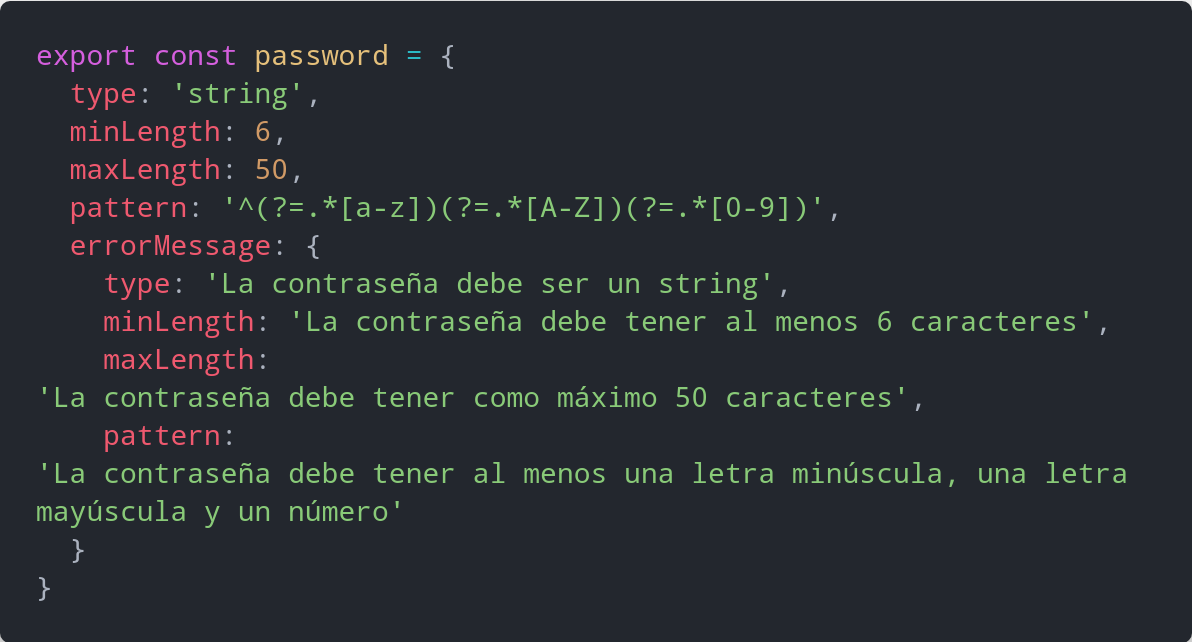
\includegraphics[width=1\textwidth]{img/password-dto}
  \caption{Definición de la propiedad \texttt{password} del DTO de inicio de sesión y registro}
  \label{fig:password-dto}
\end{figure}

Los esquemas de validación DTO se generan con una función auxiliar que se ha creado con este
propósito y se compila con la función \texttt{ajv.compile()} de la librería \textit{Ajv}
\cite{ajv-methods}. Con este esquema se crea un middleware que se ejecuta antes de las
funciones de los controladores y que se encarga de validar los datos que llegan en el body
de la request. Si los datos no son válidos, se devuelve un error con los mensajes de error
definidos en el esquema de validación correspondiente. Un ejemplo de esto se puede ver en
la imágen \ref{fig:auth-router} donde podemos ver los middlewares \texttt{validateLoginDTO}
y \texttt{validateSignUpDTO} que se ejecutan antes de las funciones \texttt{postLogin} y
\texttt{postSignUp} respectivamente.

\newpage

\subsubsection{Autenticación} \label{sssec:auth}
Para la autenticación de los usuarios en la aplicación se ha utilizado \textit{JWT}
\cite{jwt} que es un estándar basado en objetos \textit{JSON} para poder transmitir
información de forma segura y firmada digitalmente a través de un token. Se barajó la
opción de utilizar una autenticación basada en sesiones, pero se descartó porque
la autenticación mediante token es más segura y sencilla de implementar, como se
explica en este artículo \cite{token-vs-session}.

Para el manejo de los tokens se ha utilizado el módulo \textit{jose} \cite{jose} que
permite generar y verificar tokens \textit{JWT} \cite{jwt} mediante una serie de funciones.

Dado que junto con el token se puede enviar información encriptada para que el cliente
pueda acceder a ella, se ha decidido enviar el \textbf{id del usuario} y su \textbf{rol}.
Esto permite que desde el frontend se pueda saber de manera sencilla si el usuario está
autenticado y qué acciones puede realizar en la aplicación.

Para la firma del token se ha utilizado un \textit{secret} que se ha definido en una
variable de entorno en el \texttt{.env}. Este \textit{secret} se utiliza para verificar
que el token es válido y que no ha sido modificado. Todo este proceso se explica en la
documentación \cite{jose-sign}, donde se enseña también a encriptar con diferentes
algoritmos. En este caso se ha utilizado el algoritmo \texttt{HS256}. Además se ha
definido un tiempo de expiración del token de \textbf{8 horas}, tiempo tras el cual
el token dejará de ser válido y el usuario tendrá que volver a iniciar sesión.

Desde el frontend, cada vez que se realiza una petición a la API (que deba estar
autenticada), se envía el token en la cabecera de la petición siguiendo el estándar
\textit{Bearer} \cite{bearer}. Este token se verificará en el backend y, si es válido,
se ejecutará la función correspondiente de la petición, en caso contrario, se devolverá
un error de autenticación.

Para la autenticación de los usuarios se ha creado un middleware que se ejecuta antes
de las funciones de los controladores y que se encarga de verificar que el token que
llega en la cabecera de la petición es válido, utilizando la función \texttt{jwtVerify()}
\cite{jose-verify} de \textit{jose}.

Este middleware se puede ver en la imágen \ref{fig:auth-middleware}. En caso de que el
token sea válido, se obtiene el id del usuario y se añade al objeto \texttt{req}, después
se ejecuta la función \texttt{next()} para que se ejecute la función del controlador
correspondiente a la petición, donde se podrá acceder al id del usuario que se acaba de
almacenar en \texttt{req}. Si el token no se válido se envía el error de autenticación
con la función \texttt{next()} para que se ejecuten los middlewares de manejo de errores
explicados anteriormente.

\begin{figure}[H]
  \centering
  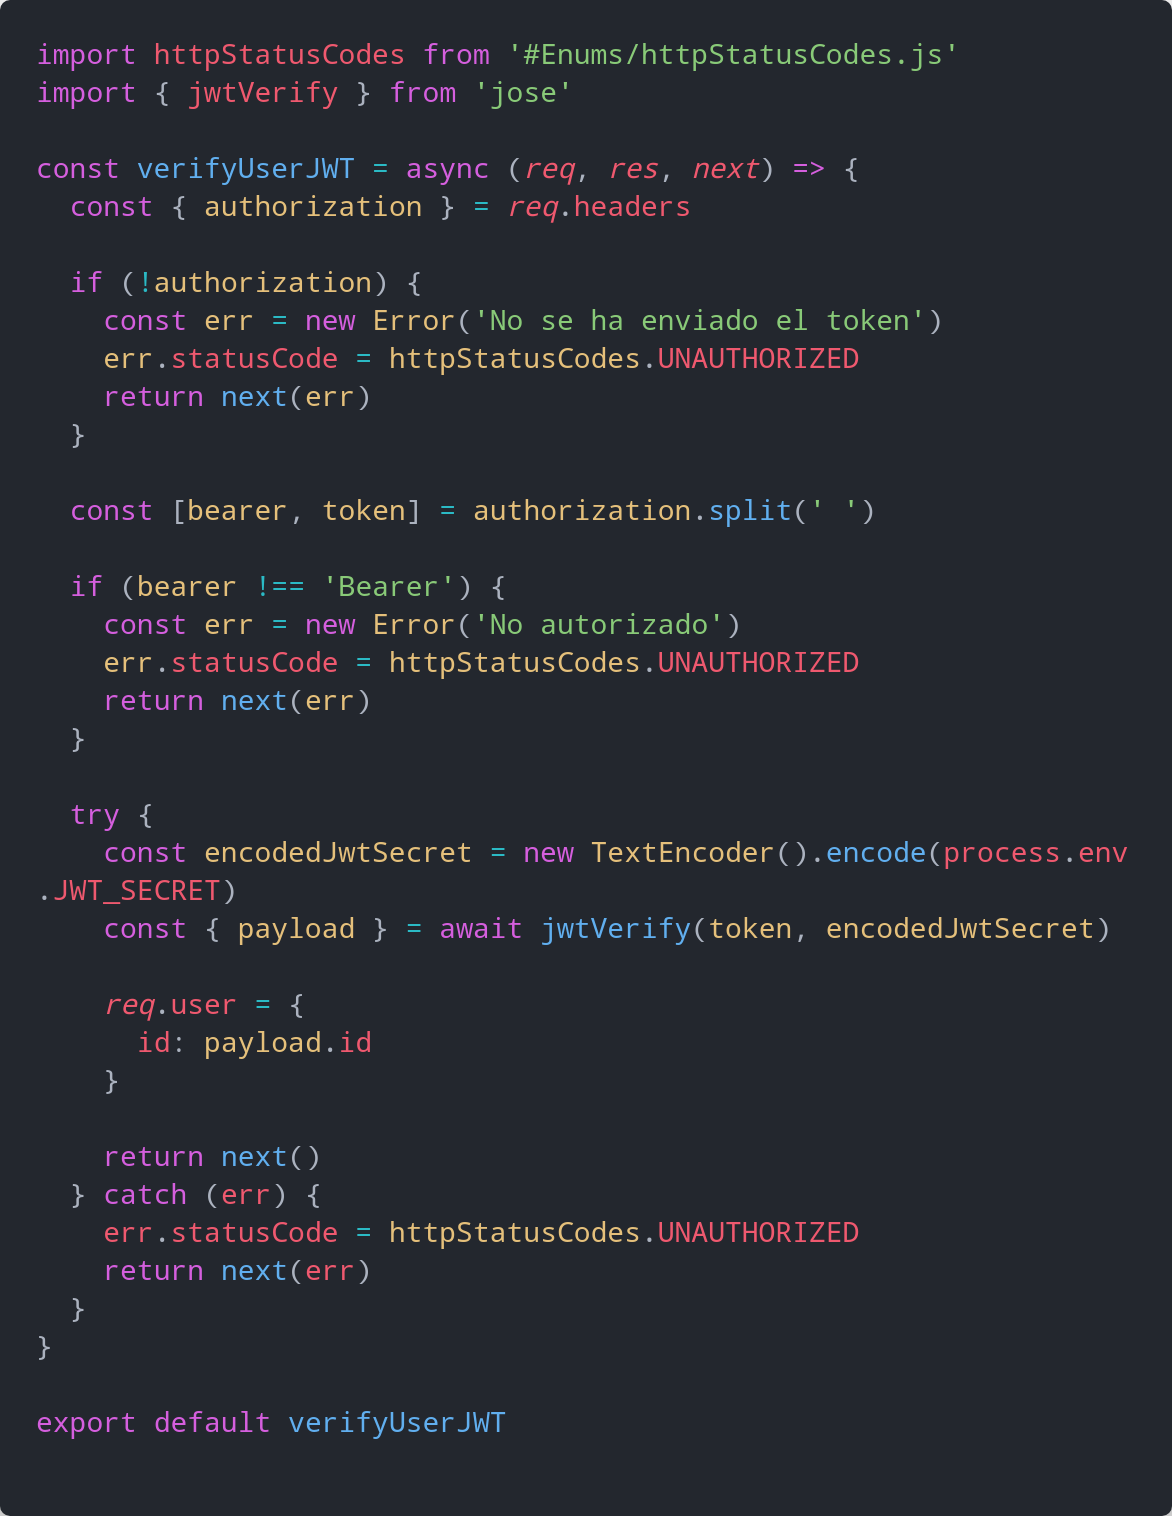
\includegraphics[width=0.8\textwidth]{img/auth-middleware}
  \caption{Middleware de autenticación}
  \label{fig:auth-middleware}
\end{figure}

\subsection{Frontend}

El frontend de la aplicación se ha desarrollado utilizando \textit{React} \cite{react}
y algunos componentes de \textit{Material-UI} \cite{material-ui}.

La aplicación de \textit{React} \cite{react} consta de un archivo \texttt{index.html}
que es el punto de entrada de la aplicación y donde se encuentra el elemento
\texttt{<div id=``root''></div>} en el cual se va a renderizar la aplicación. A nivel de
\textit{JavaScript} se tiene un archivo \texttt{main.jsx} que es el archivo desde el que
se inicia la aplicación y donde, a través del react-dom, se obtiene el elemento
\texttt{<div id=``root''></div>} mencionado anteriormente y en él se renderiza el componente
\texttt{App} que es el componente principal de la aplicación.

\subsubsection{Vite}

Para hacer el frontend de la aplicación se ha creado un proyecto nuevo usando
\textit{Vite} \cite{vite} que es una herramienta que facilita el desarrollo del frontend
de aplicaciones web. Consta de un servidor de desarrollo para poder ir viendo los cambios
que se van realizando en la aplicación en tiempo real y de un \textit{bundler} que se
encarga de compilar el código con todas sus dependencias.

Se ha utilizado \textit{Vite} \cite{vite} en lugar de \textit{Create React App}
\cite{create-react-app}, que era la herramienta que se utilizaba anteriormente por defecto
para crear proyectos de \textit{React} \cite{react}, porque es más rápido y por su
manejo de las dependencias. Además, en la documentación oficial de \textit{React}
\cite{start-react-project} ahora recomienda utilizar \textit{Vite} \cite{vite} para crear
nuevos proyectos si no vamos a utilizar un framework completo.

En las imágenes \ref{fig:vite-bundle} y \ref{fig:vite-esm} \cite{why-vite} se puede ver la
diferencia entre lo que se hace tradicionalmente con \textit{bundlers} para el desarrollo y
lo que hace \textit{Vite} \cite{vite}, que es utilizar el sistema de módulos de JavaScript
(\textit{ESM}) \cite{esm} para importar los módulos dinámicamente en el navegador. Esto
agiliza mucho el proceso de desarrollo evitando tener que compilar el código cada vez que
se realiza un cambio.

\begin{figure}[H]
  \centering
  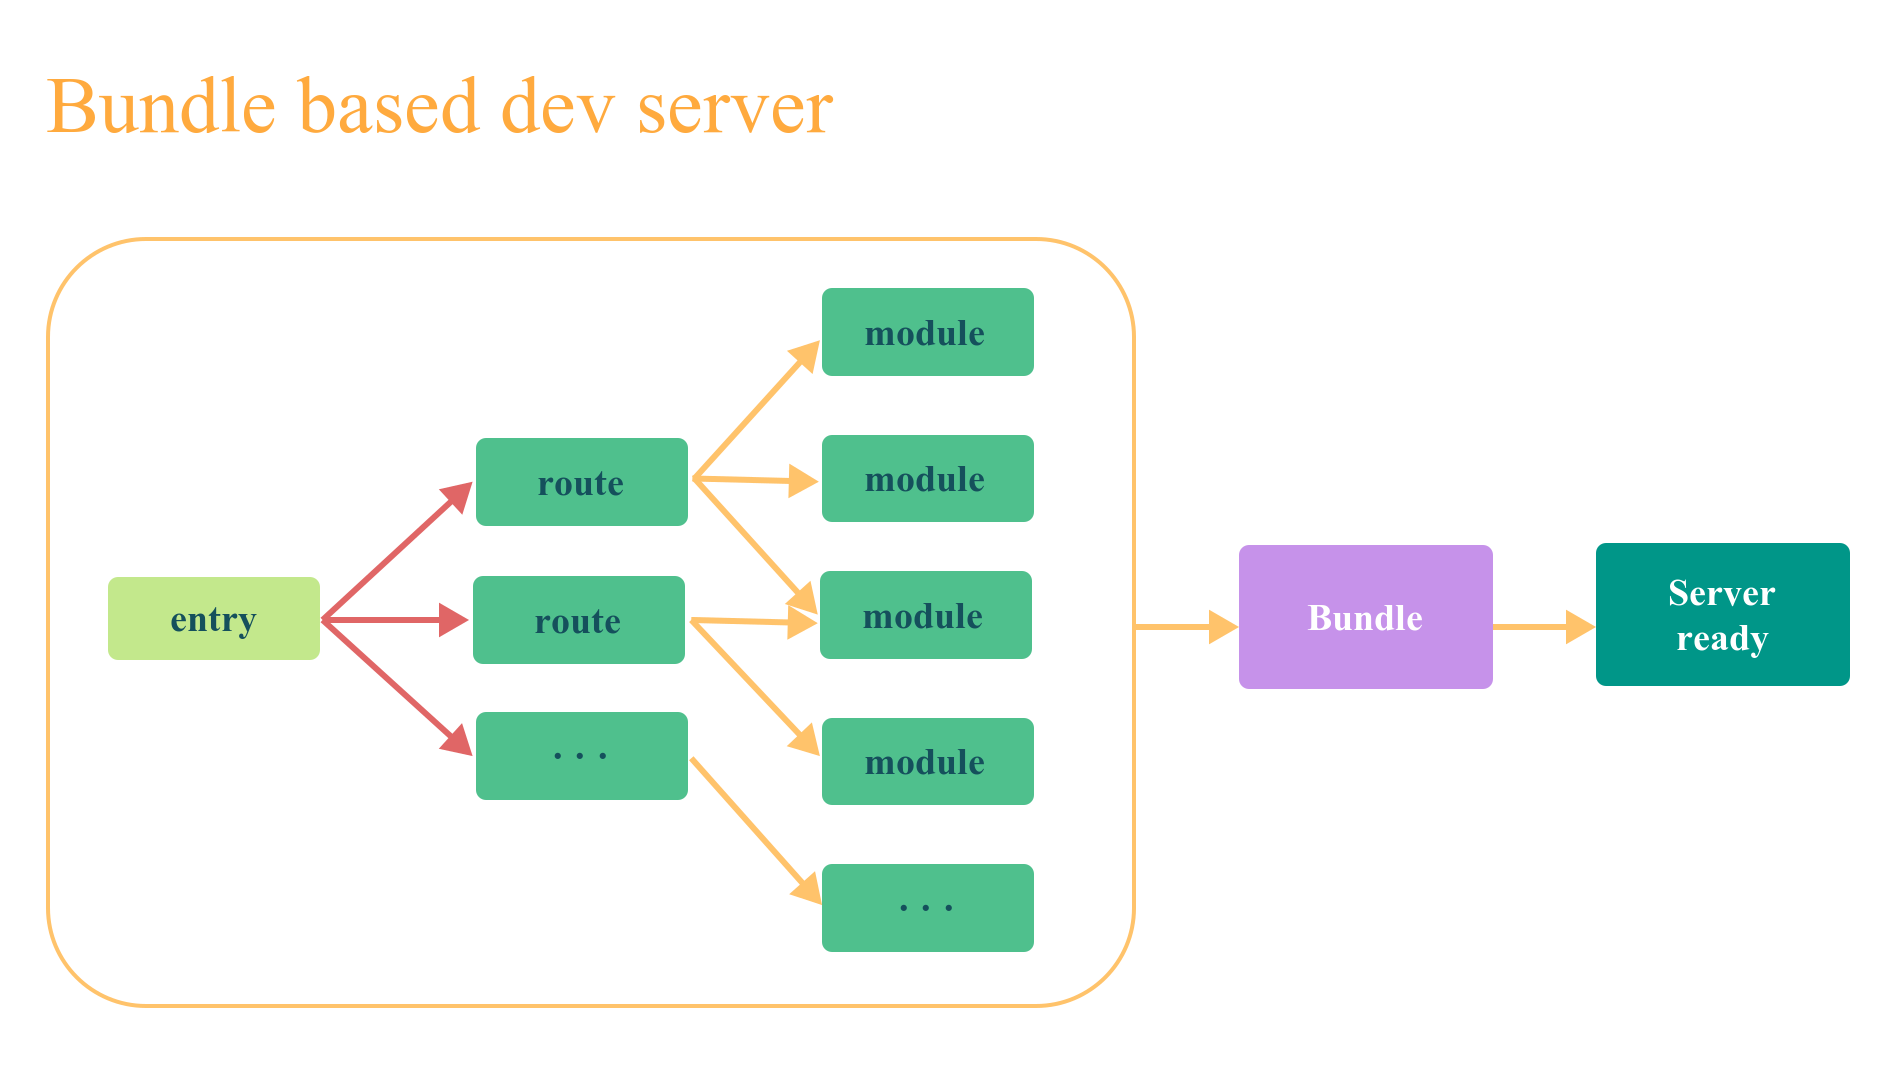
\includegraphics[width=1\textwidth]{img/bundle-based}
  \caption{Proceso de desarrollo con \textit{bundlers} \cite{why-vite}}
  \label{fig:vite-bundle}
\end{figure}

\begin{figure}[H]
  \centering
  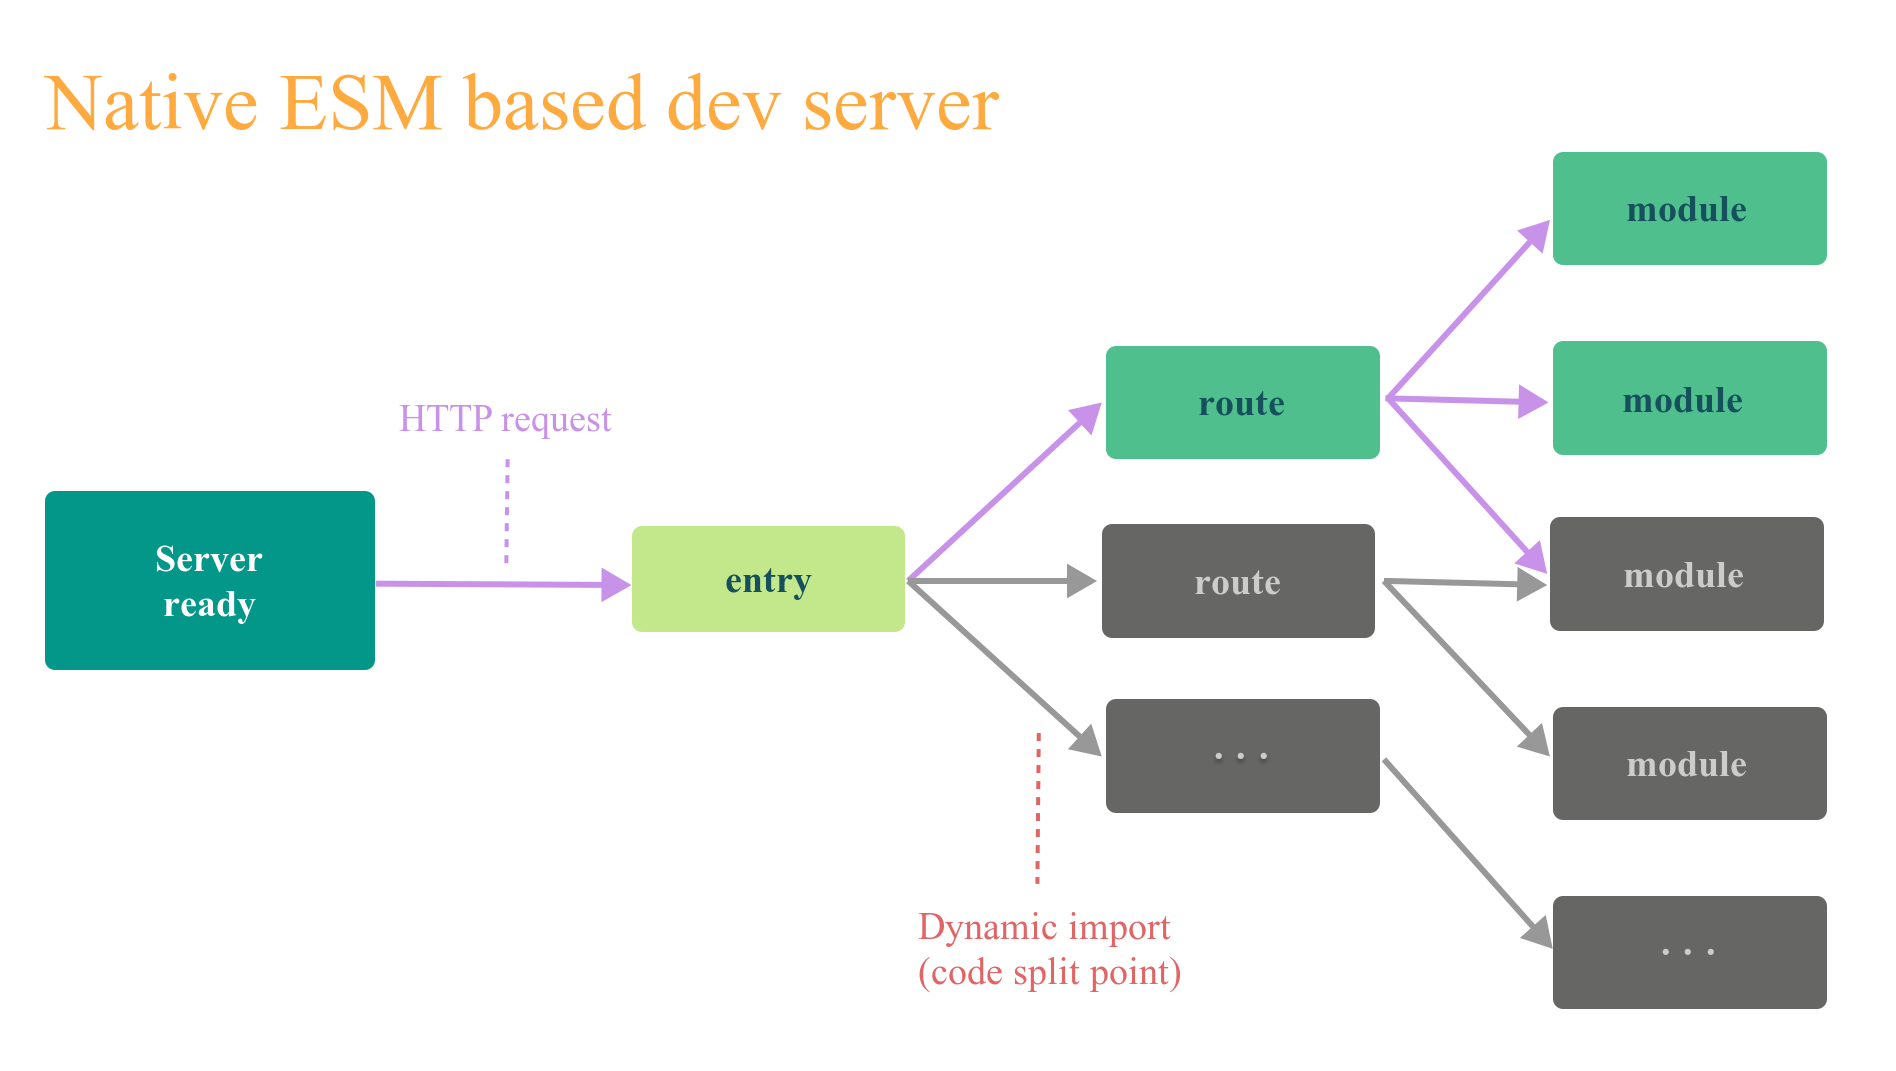
\includegraphics[width=1\textwidth]{img/esm-based}
  \caption{Proceso de desarrollo con \textit{ESM} \cite{why-vite}}
  \label{fig:vite-esm}
\end{figure}

Se ha utilizado también \textit{SWC} \cite{swc} que es un compilador de JavaScript y
TypeScript que es más rápido que \textit{Babel} \cite{babel} y que se integra con
\textit{Vite} \cite{vite} con un plugin que han desarrollado \cite{vite-swc}, afirmando
que es hasta 20 veces más rápido que \textit{Babel} \cite{babel}.

\subsubsection{Rutas}
Para gestionar las rutas de la aplicación se ha utilizado \textit{React Router}
\cite{react-router} que es la librería más utilizada para este propósito.

Se ha usado el componente \texttt{BrowserRouter} y se ha seguido la documentación
\cite{browser-router} para definir las rutas de la aplicación. En la imágen
\ref{fig:app} se puede ver el componente \texttt{App} que es el componente principal
de la aplicación y donde se definen las rutas de la misma.

Como se puede observar, se define el \texttt{AuthProvider} (que se explicará más adelante)
y dentro de él se define el componente \texttt{Routes} que es el que se encarga de
definir las rutas de la aplicación.

La primera ruta tiene \texttt{path='/'}, que es la ruta raíz por lo que todas las rutas
renderizarán el componente que se le pasa como valor a la prop \texttt{element}, el
componente \texttt{Layout}. Este componente es el que tiene la estructura principal de la
aplicación, que tiene que estar presente en todas las páginas. Consta de un \texttt{header}
con la barra de navegación y un \texttt{main} donde se renderiza el componente
\texttt{Outlet} \cite{outlet} que se encarga de renderizar el \texttt{element}
correspondiente a la ruta hija que se esté visitando.

La última ruta, con \texttt{path='*'}, es la ruta por defecto que se renderiza cuando
no se encuentra ninguna otra ruta que conicida con la ruta que se está visitando en la
aplicación.

\newpage

\begin{figure}[H]
  \centering
  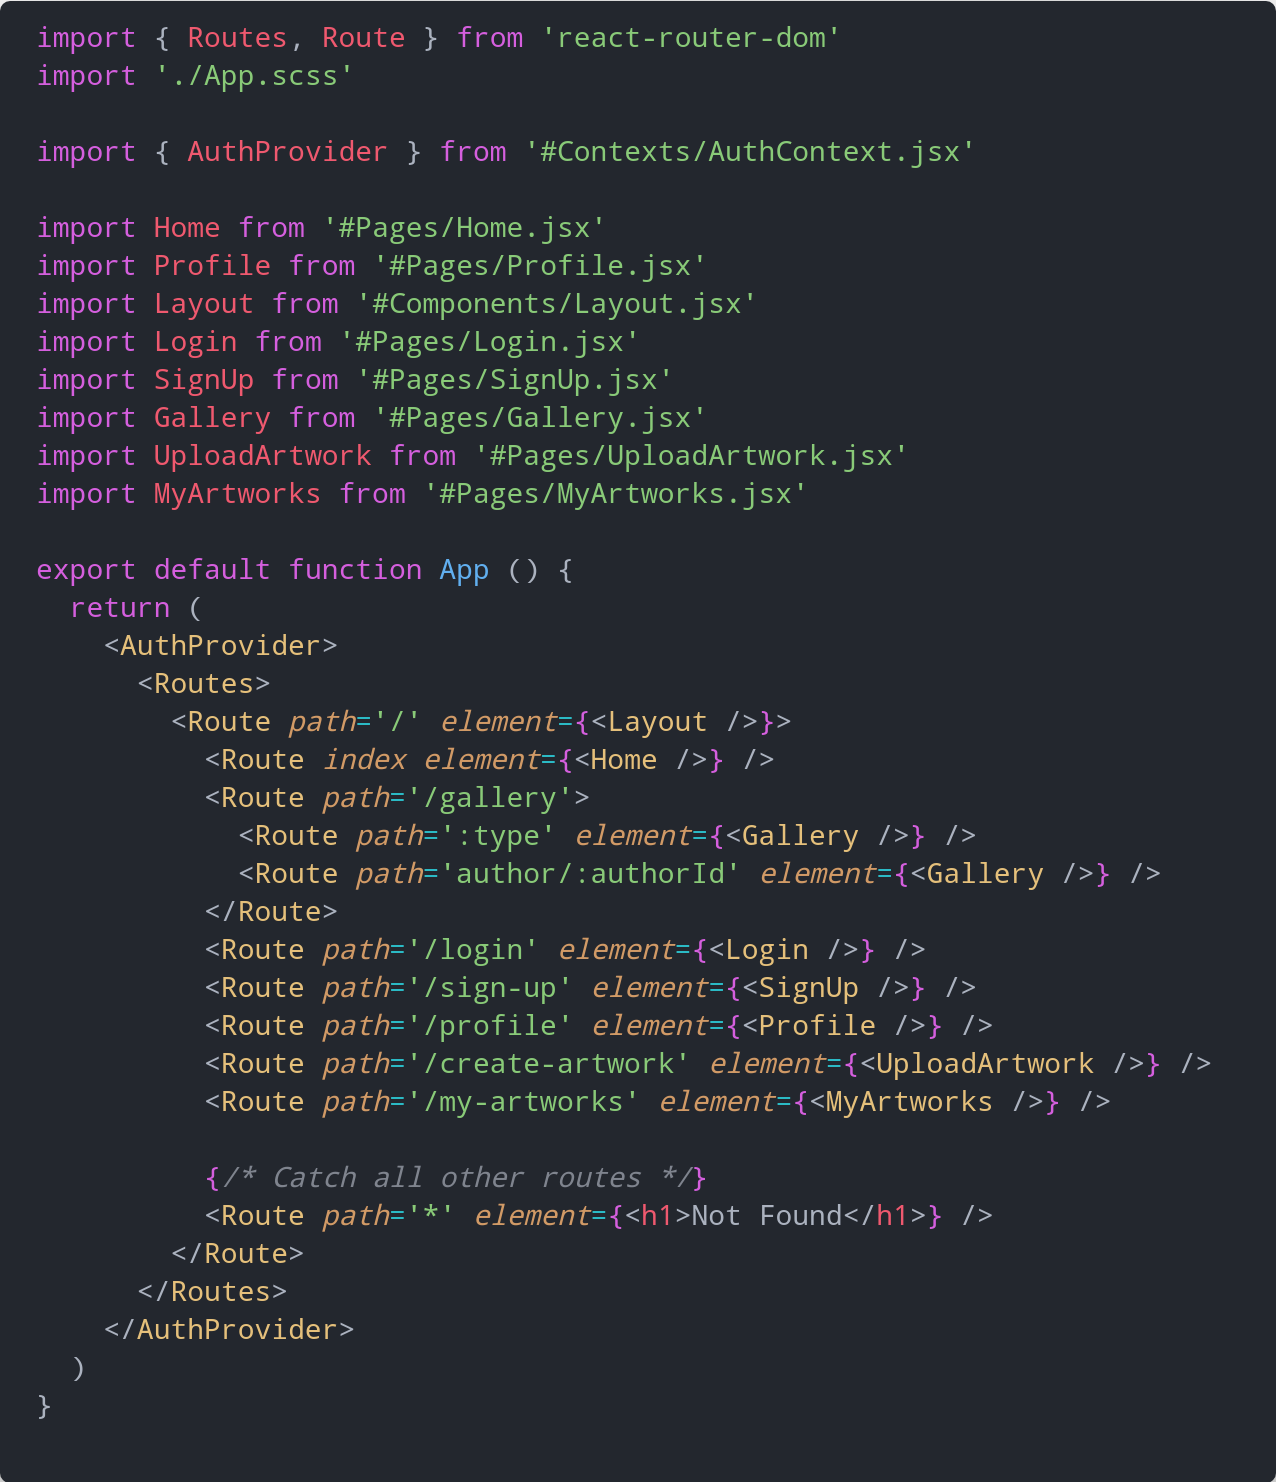
\includegraphics[width=1\textwidth]{img/app}
  \caption{Componente \texttt{App}}
  \label{fig:app}
\end{figure}

\newpage

\subsubsection{Contexto de autenticación} \label{sssec:AuthContext}
Para gestionar la autenticación de los usuarios en el frontend se ha utilizado el
\textit{hook} \texttt{useContext} \cite{use-context} de \textit{React} \cite{react},
que permite suscribirse a un contexto previamente definido y acceder a él desde cualquier
componente hijo de dicho contexto.

Para esto se ha definido el contexto \texttt{AuthContext} con la función
\texttt{createContext} \cite{create-context} de \textit{React} \cite{react} y se ha creado
un componente \texttt{AuthProvider} que es el que se encarga de gestionar el estado de la
autenticación de los usuarios. Este es el que se puede ver en la imágen \ref{fig:app}
englobando al resto de componentes de la aplicación. Esto permite que este contexto esté
disponible en toda la aplicación.

En el componente \texttt{AuthProvider} se definen los estados \texttt{user} y
\texttt{token} que son los que se van a utilizar para guardar la información de
autenticación del usuario, en caso de ser nulos, significa que el usuario no está
autenticado. También se definen las funciones \texttt{setAuth} y \texttt{deleteAuth} que
se encargan de guardar y eliminar la información de autenticación del usuario en el
\textit{localStorage} \cite{local-storage} del navegador.

\subsubsection{Componentes}
Los \textbf{componentes} son la base que utiliza \textit{React} \cite{react} para
construir las interfaces de usuario \cite{react-component}. Los componentes son como
funciones que engloban el marcado \textit{HTML}, los estilos \textit{CSS} y la lógica
\textit{JavaScript} de una parte concreta de la interfaz de usuario. Los componentes
devuelven un código \textit{JSX} \cite{jsx} muy similar al \textit{HTML} y es el que
se renderiza en el navegador. Los componentes pueden tener propiedades que se pasan
como parámetros desde el componente padre.

En la aplicación se han creado algunos \textbf{componentes} en la carpeta \texttt{pages}
que son los que se renderizan al visitar una ruta de la aplicación. Estos componentes
suelen ser componentes padres que engloban a otros componentes más pequeños que se
encargan de renderizar partes más concretas de la página. Estos componentes más pequeños
se han creado en la carpeta \texttt{components} y también pueden tener componentes hijos
que se renderizan dentro de ellos.

Para manejar la lógica de los componentes se han utilizado los \textbf{estados} de
\textit{React} \cite{react-state} que son como variables de los componentes que se
mantienen entre renderizados y que, al ser modificados, hacen que el componente se
vuelva a renderizar, permitiendo así que se actualice la interfaz de usuario.

\subsubsection{Estilos}
Para los estilos de la aplicación se han escrito en \textit{SCSS} \cite{scss} y se han
utilizado algunos componentes de \textit{Material-UI} \cite{material-ui} como, por ejemplo,
el componente \texttt{Rating} \cite{rating} para mostrar las valoraciones de las obras o
el componente \texttt{Modal} \cite{modal} que se utiliza para mostrar los detalles de una
obra de arte de la galería. Además, este último componente se ha anidado dentro de otro
\texttt{Modal} para mostrar todas las valoraciones y comentarios de una obra de arte.

\subsubsection{Hooks}
Los \textbf{hooks} son una característica de \textit{React} \cite{react-hooks} que
permite usar distintas funciones de \textit{React} \cite{react} en los componentes.
Por ejemplo el \textit{hook} \texttt{useState} \cite{use-state} para manejar los
\textit{estados} de los que se ha hablado anteriormente o el \textit{hook}
\texttt{useContext} \cite{use-context} para poder acceder a un contexto como se ha
explicado en la sección anterior, sobre el contexto de autenticación \ref{sssec:AuthContext}.

Además, \textit{React} \cite{react} permite crear \textbf{hooks personalizados} que
llaman \textbf{custom hooks} \cite{custom-hooks}. Estos permiten encapsular una lógica
que se vaya a utilizar en varios componentes. En la aplicación se han creado algunos
\textbf{custom hooks} como el hook \texttt{useAuth} que se encarga de obtener la
información de autenticación del usuario del contexto de autenticación o el hook
\texttt{useErrors} que se encarga de gestionar los errores que se pueden producir en los
componentes. Este último se muestra en la imágen \ref{fig:use-errors} donde se puede ver
que se define un estado \texttt{errors} para almacenar los errores y dos funciones:
\texttt{saveErrors} que se encarga de guardar los errores en el estado y \texttt{clearErrors},
encargada de limpiar los errores del estado.

\begin{figure}[H]
  \centering
  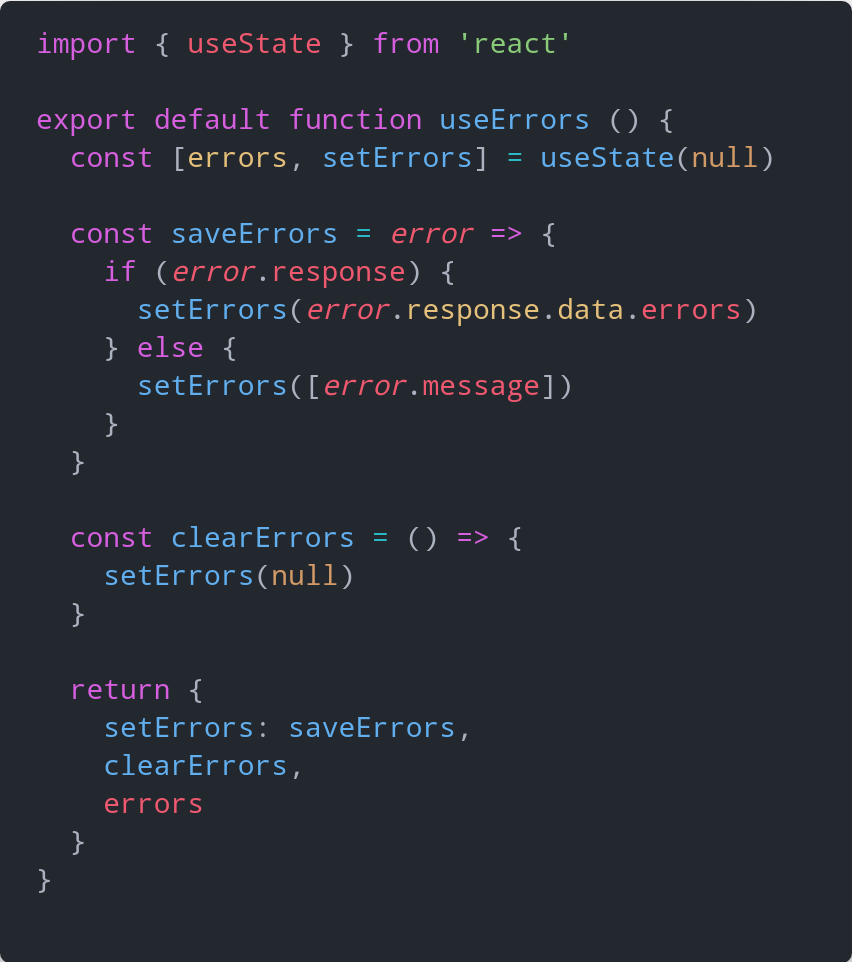
\includegraphics[width=0.6\textwidth]{img/use-errors}
  \caption{Hook \texttt{useErrors}}
  \label{fig:use-errors}
\end{figure}

\subsubsection{Servicios}
Para realizar las peticiones \texttt{HTTP} a la API se han creado unos servicios que
se encargan de esta labor. Se han creado tres servicios, uno para las peticiones relacionadas
con la autenticación, otro para las peticiones relacionadas con los usuarios y otro para
las relacionadas con las obras de arte.

Las peticiones se realizan mediante la librería \textit{Axios} \cite{axios} que permite
realizar peticiones \texttt{HTTP} de manera sencilla. La configuración de \textit{Axios}
\cite{axios} es muy sencilla, simplemente se crea una instancia indicando la \texttt{baseURL}
de la API. Esto se ha realizado en un archivo de configuración \texttt{axios.js} que devuelve
la instancia del cliente de \textit{Axios} \cite{axios} evitando así tener que crear una
instancia en cada servicio.

La instancia de \textit{Axios} \cite{axios} cuenta con los métodos \texttt{get},
\texttt{post}, \texttt{put} y \texttt{delete} que son los que se utilizan para realizar
las peticiones \texttt{HTTP} a la API. A estos métodos hay que pasarles como primer
parámetro la ruta de la petición, como segundo parámetro los datos que se quieran enviar
en el body de la petición (en caso de que sea necesario) y el último parámetro es un objeto
con la configuración de la petición como, por ejemplo, los \textit{headers}.

En la imágen \ref{fig:create-artwork-service} se puede ver la función \texttt{createArtwork}
del servicio de obras de arte que se encarga de realizar una petición \texttt{POST} a la API
para crear una obra de arte. En ella se puede ver que la función recibe como parámetro un
objeto con los datos de la obra de arte y el token de autenticación del usuario. Se utiliza
el método \texttt{post} de la instancia de \texttt{axiosClient} pasándole como primer
parámetro la ruta de la petición, como segundo los datos con los que se quiere crear la obra
de arte y como tercer parámetro los \textit{headers} de la petición, que en este caso son
el \textit{header} de \texttt{Authorization} con el token en el formato \texttt{Bearer}, tal
y como se explicó en la sección \ref{sssec:auth}; y el \textit{header} de
\texttt{'Content-Type': 'multipart/form-data'} que es el que se recomienda cuando se envían
datos con archivos, como es el caso de las obras de arte \cite{multipart-form-data}. Por
último, se devuelve la respuesta de la petición.

\begin{figure}[H]
  \centering
  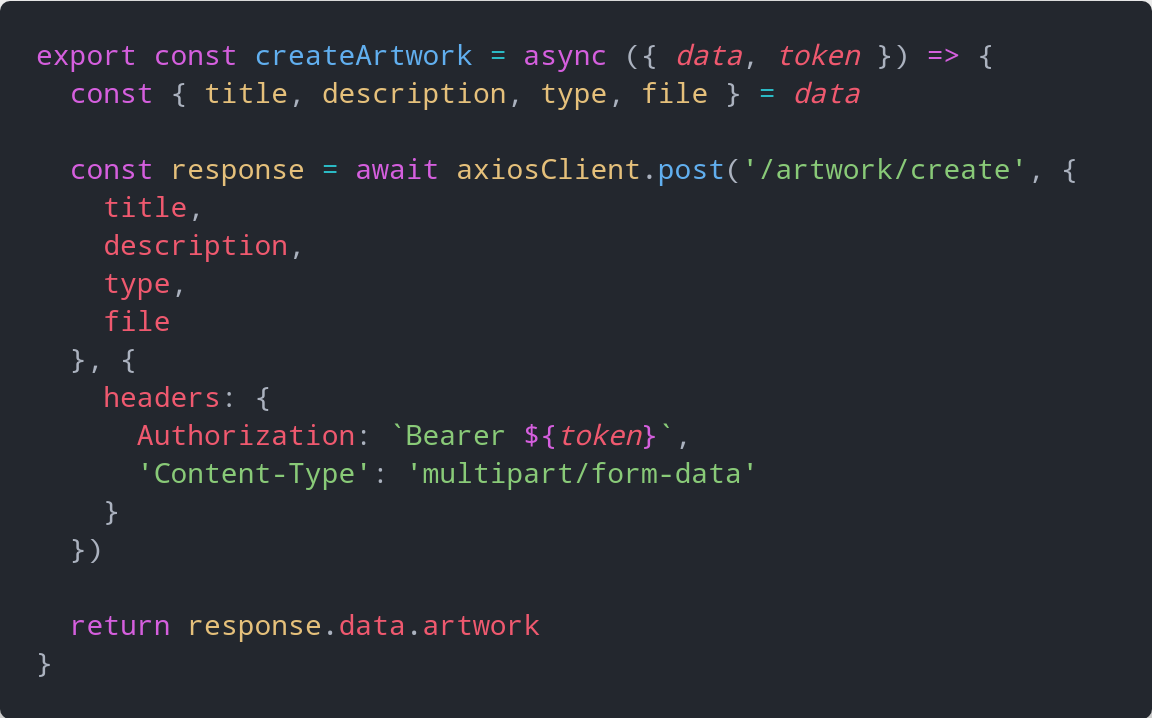
\includegraphics[width=1\textwidth]{img/create-artwork-service}
  \caption{Función \texttt{createArtwork}}
  \label{fig:create-artwork-service}
\end{figure}

\subsection{Despliegue}
Para el despliegue y conexión de todas las partes de la aplicación se ha utilizado
\textit{Docker} \cite{docker} que es una plataforma que permite crear, desplegar y ejecutar
aplicaciones dentro de contenedores. Estos contenedores son un \textbf{entorno de
virtualización} ligero y aislado que permite ejecutar aplicaciones independientemente del
sistema operativo en el que se ejecute. A diferencia de una máquina virtual, los contenedores
no necesitan un sistema operativo virtualizado para funcionar, sino que utilizan los recursos
del sistema operativo del host y solamente virtualizan los componentes necesarios para
ejecutar la aplicación y sus dependencias. Estos contenedores son \textbf{independientes del
sistema operativo} y entre ellos, por lo que podemos evitar así problemas de dependencias o
conflictos entre aplicaciones aunque se ejecuten en el mismo host.

Para el despliegue de la aplicación se ha utilizado \textit{Docker Compose}
\cite{docker-compose} que permite definir y ejecutar multiples contenedores de \textit{Docker}
\cite{docker}. En el caso de esta aplicación, se han definido cuatro contenedores: uno para
la base de datos, otro para \textit{PhpMyAdmin} \cite{phpmyadmin}, otro para el backend y
otro para el frontend.

Tanto el backend como el frontend se han definido con un \textit{Dockerfile} \cite{dockerfile}
que es un archivo que contiene instrucciones para crear una \textit{imagen} de \textit{Docker}
para crear el contenedor. En ambos, se ha utilizado como base la \textit{imagen} oficial
de \textit{Node.js} \cite{nodejs-docker} en su versión \texttt{18-alpine} que está basada en
\textit{Alpine Linux} \cite{alpine-linux} (una distribución muy ligera de Linux). Además,
en estos \textit{Dockerfiles} se copian los archivos necesarios del host de la aplicación al
contenedor y se instalan las dependencias de la aplicación con el comando \texttt{npm install}
de \textit{npm} \cite{npm}.

La base de datos se ha definido directamente en el \textit{docker-compose.yml} usando la
\textit{imagen} oficial de \textit{MySQL} \cite{mysql-docker} en su versión \texttt{8.0}
y definiendo las variables de entorno necesarias para la configuración de la misma.

Para el gestor de base de datos se ha utilizado la \textit{imagen} oficial de
\textit{PhpMyAdmin} \cite{phpmyadmin-docker} en su última versión y también se han definido
las variables de entorno necesarias para su conexión con la base de datos.

	
	\chapter{Pruebas}

{ \setlength{\parskip}{6mm} % Customize the space between paragraphs
Las pruebas de la aplicación se han realizado a lo largo del desarrollo de la misma. Se ha
ido probando cada funcionalidad conforme se iba implementando.

Durante el proceso de implementación había funcionalidades que se probaron y no se
encontró ningún error, pero cuando se terminó de implementar la aplicación y se volvieron
a probar todas las funcionalidades y casos de uso de la aplicación, se encontraron errores
que no se habían detectado anteriormente.

Un ejemplo de esto es el caso de uso de subir una obra de arte. Cuando se implementó
esta funcionalidad se probó y no se encontró ningún error, pero cuando se terminó de
implementar la aplicación y se volvió a probar, se encontró el error. La descripción
de la obra tenía un límite de 500 caracteres en las comprobaciones que se hacían mediante
el sistema de DTO, pero en base de datos, este límite era de 200 caracteres. Esto provocaba
que si se introducía una descripción de más de 200 caracteres, saltase un error de la base de
datos en lugar de un error personalizado de la aplicación.

Se han realizado las pruebas de todas las funcionalidades tanto conforme se iban
implementando como al finalizar la implementación de la aplicación y en la fase de
implementación sí es cierto que se encontraron bastantes errores que se fueron corrigiendo,
pero en la fase final de pruebas, estaba todo más depurado y se encontraron menos errores.

En un futuro, si la aplicación se sigue desarrollando y se lanza a producción, se deberían
realizar pruebas unitarias y de integración para asegurar que la aplicación funciona
correctamente y que no se introducen errores al realizar cambios en el código.
}

	% Presupuesto

	% Conclusiones
	\chapter{Conclusiones y trabajos futuros}



	% Trabajos futuros


	
	\newpage
	\bibliography{bibliografia}
	\bibliographystyle{plain}
	
\end{document}

